% Version 21-02-2020
% update 14-11-2016 by Ken Arroyo Ohori: 
% made spacing closer to Word template throughout,
% put proper quotes everywhere,
% removed spacing that could cause labels to be wrong, 
% added non-breaking and inter-sentence spacing
% where applicable, removed explicit newlines
% 21.2.18: m. sester: changed Creative Commons 3.0 License to 4.0, 
% adaption to ICA-Proceedings
% 21-02-2020: Juergen Bierwirth: correction of header size/margins

\documentclass{ica}
%\PassOptionsToPackage{hyphens}{url}
\usepackage{hyperref}
\hypersetup{
    colorlinks=true,
    linkcolor=blue,
    filecolor=blue,      
    urlcolor=blue,
    citecolor=blue
}

\usepackage{xurl} %make a link to break at the page margin
%\usepackage{subfigure}
\usepackage{setspace}
\usepackage{geometry} % added 27-02-2014 Markus Englich
\usepackage{epstopdf}
% added 14-04-2016 Markus Englich - Recommendation by Sebastian Brocks
\usepackage[labelsep=period]{caption} 
\usepackage{blindtext}
\graphicspath{{images/}}

\usepackage{subcaption} %for \subfigure
\usepackage{booktabs} %for \toprule

\usepackage{amsmath} %for \begin{equation*}\end{equation*}


%\usepackage{multicol}


\geometry{a4paper, top=25mm, left=20mm, right=20mm, bottom=28mm}
% added 27-02-2014 Markus Englich; bottom changed to 28mm by Juergen Bierwirth
%\usepackage{enumitem}

%\renewcommand*{\thefootnote}{\fnsymbol{footnote}}
%\captionsetup{justification=centering} % thanks to Niclas Borlin 05-05-2016


%\usepackage[headsepline,plainheadsepline]{scrlayer-scrpage}
\usepackage{fancyhdr}
\usepackage{natbib}% Citation support using natbib.sty
\usepackage{xspace}

\fancyhf{}
\lhead{}
\rhead{}
%\chead{\thenumber}

\fancypagestyle{first}{%
    \fancyhead[L]{
\includegraphics[height=1.15cm]{ica-logo.pdf}}
    \fancyhead[R]{}
    \renewcommand{\headrulewidth}{0.4pt}
}

% pagination in header from 2nd page onwards
% changed 13-03-2018 by Juergen Bierwirth: 
% 'page number' to 'page number' of 'number of total pages' of the document
\fancyhead[EL,OR]{\fontfamily{\sfdefault}
    \footnotesize\selectfont\thepage~of~\pageref{LastPage}{\vskip 18pt}} 
\renewcommand{\headrulewidth}{0pt}
%\fancyhead[EL]{\thepage}

\newcommand{\Astar}{A$^{\!\star}$\xspace}

\newcommand{\e}[1]{\times 10^{#1}}
\newcommand{\fig}{Figure~}
\newcommand{\eq}{Equation~}
\newcommand{\fo}{Formula~}
\newcommand{\sect}{Section~}
\newcommand{\tabl}{Table~}
\newcommand{\tabls}{Tables~}
\newcommand{\tbl}{Table~}
\newcommand{\tbls}{Tables~}
\newcommand{\chap}{Chapter~}
\newcommand{\figs}{Figures~}
\newcommand{\eqs}{Equations~}
\newcommand{\fos}{Formulas~}
\newcommand{\sects}{Sections~}
\newcommand{\appx}{Apendix~}

\newcommand{\chaps}{Chapters~}
\newcommand{\p}{p.~}
\newcommand{\pp}{pp.~}
\newcommand{\eg}{e.g.,}
\newcommand{\ie}{i.e.,}

\pagestyle{fancy}

%\newcommand*\varhrulefill[1][0.4pt]
%   {\leavevmode\leaders\hrule height#1\hfill\kern0pt}


%---------------------------------------------------------------------------------
% authors: begin your individual input here!

\begin{document}
\title{Paralleling generalization operations to support smooth zooming:
case study of merging area objects}

\author{
 Dongliang Peng\,\thanks{Corresponding author} , 
 Martijn Meijers, Peter van Oosterom}

\address{
 Section GIS Technology, Faculty of Architecture and the Built Environment,
 Delft University of Technology, Delft, The Netherlands, 
 \{D.L.Peng, B.M.Meijers, P.J.M.vanOosterom\}@tudelft.nl\\
}

% If the corresponding author is NOT the final author, 
% always add a space before the subsequent comma, i.e.
% first author name\textsuperscript{a,}\thanks{Corresponding author} , 
% second author name \textsuperscript{b}, etc.
% thanks to Niclas Borlin 05-05-2016

\abstract{
When users zoom out on a digital map, 
some area objects become too tiny to be seen, 
resulting in visual clutters. 
To avoid this problem, 
the relatively unimportant areas should be merged
with their neighbors to form larger areas.
In order to provide small and smooth changes
so that users can easily keep their contexts,
we merge a pair of areas by expanding one over the other
and parallel the merging operations.
We also require that the area objects 
involved in paralleled merging operations
should not have any common neighbor
so that the topology of the map can be easily maintained.
The zooming of our map is realized based on the
topological area partitioning tree (GAP-tree)
and the space-scale cube (SSC).
Our case study shows that
our method can improve the zooming visualization.
We consider that paralleling generalization operations
is an important step towards continuous map generalization.
%However, if several areas are merged into an area in a single operation,
%then it is a large and discrete change, 
%which confuse map users.
%In order to provide small and smooth changes,
%this paper merges a pair of areas by expanding one over the other
%and parallel the merging operations.
%However, if the changes happen sequentially,
%then the changes have to happen very fast 
%because the map user wants to see the map at the target scale 
%rather soon after applying a zooming operation.
%In order to allow each change has more time to take place, 
%we propose to parallel the merging operations.
%This paper shows the details of finding and processing parallel merging operations.
%We consider that parallel generalization operations
%is an important step towards continuous map generalization. 
}

\keywords{Space-scale cube,  
vario-scale map, continuous map generalization}
%\\ \hline


\maketitle

\thispagestyle{first}

%\saythanks % option for xx

\section{Introduction}

When users are reading a digital map,
they expect different levels of detail (LoDs) depending on the scales.
For example, they may want to see individual buildings when zooming in
and see built-up areas when zooming out.
That is why geographical information is dependent on the scale
\citep{Muller1995Generalization,Weibel1997}. 
In order to prepare map data for different scales,
a detailed map is generalized to generate coarser data 
for maps at smaller scales,
which is known as map generalization.
%A lot of research has been devoted to map generalization.
\citet{Mackaness2017Generalization} gave a taxonomy of 
generalization algorithms, 
including selection, simplification, aggregation, and so on.
Often, a multi-representation database (MRDB) is utilized to store
maps at different scales and to send proper data to clients on request
\citep[\eg][]{Hampe2004multiple}.
However, large and discrete changes between different map representations
may confuse users,
so continuous map generalization (CMG) is needed to
provide the vario-scale map with smooth scale transition.
Algorithms of CMG have been proposed 
to morph raster maps
\citep[\eg][]{Pantazis2009a}, 
to morph polylines
\citep[\eg][]{Noellenburg2008,Deng2015,Li2017Annealing},
to generalize buildings
\citep[\eg][]{Li2017_Building,Touya2017Progressive},
to transform road networks or river networks
\citep[\eg][]{Suba2016Road,Chimani2014Eat,Huang2017Matrix},
and to transform administrative boundaries
\citep[\eg][]{Peng2016Admin}.

%\citep[\eg][]{Pantazis2009a,Pantazis2009b}, 
%to morph polylines
%\citep[\eg][]{Noellenburg2008,Peng2013LSA,Deng2015,Li2017Annealing,Li2018Fourier},
%to generalize buildings
%\citep[\eg][]{Li2017_Building,Peng2017Building,Touya2017Progressive},
%to transform road networks or river networks
%\citep[\eg][]{Suba2016Road,Chimani2014Eat,Huang2017Matrix,Peng2012River},
%and to transit administrative boundaries
%\citep[\eg][]{Peng2016Admin}.




%Indeed, there are already many algorithms 
%for continuous map generalization.
%To adapt them into a web environment still needs a lot of effort.
%This paper contributes to merging area objects 
%in a web environment. 


Area objects are important features on maps. 
When users zoom out,
some area objects become too tiny to be seen,
which results in visual clutter.
The clutter can be avoided by generalizing the 
area objects.
The generalization operators include
merging \citep[\eg][]{HaunertWolff2010AreaAgg}, 
aggregating \citep[\eg][]{Shen2019Aggregation}, 
amalgamating \citep[\eg][]{Regnauld2007Amalgamation}, 
splitting \citep[\eg][]{Meijers2016Split}, 
and collapsing \citep[\eg][]{Haunert2008Skeleton}.
%\textbf{area objects can be merged, aggregated, split, collapsed}
%For example, \citet{haunert2008f} developed a method based on
%mixed-integer programming to merge area objects
%for a map at a certain scale.
However, if zooming is realized by switching between
some levels of map representations, 
large and discrete changes usually happen.
This kind of changes may cause users to lose track of
their area objects of interest \citep{vanKreveld2001}.
In order to solve this problem, 
we smoothly and parallelly generalize the area objects.

This paper is organized as follows.
\sect\ref{sec:realted_work} reviews some related work.
Our methodology is presented in \sect\ref{sec:methodology},
followed by a case study in \sect\ref{sec:case_study}.
Finally, \sect\ref{sec:concluding_remarks} draws the conclusion
and present our future work.




%which is the first time that the parallelization 
%is explicitly proposed.
%The parallel merging operations must be well distributed,
%which pushes the boundaries of tGAP and the SSC.
%Because of the parallelization, 
%we need to snap to the scales with completed generalization operations
%and need to discuss the animation time gained for each generalization operation.

%
%\begin{figure}
%\centering
%\begin{subfigure}[t]{0.48\textwidth}
%\centering
%\includegraphics[page=4,width=0.95\linewidth]{methodology}
%\caption{}
%\end{subfigure}
%\hfill
%\begin{subfigure}[t]{0.48\textwidth}
%\centering
%\includegraphics[page=5,width=0.95\linewidth]{methodology}
%\caption{}
%\end{subfigure}
%\caption{
%
%}
%\label{fig:ssc}
%\end{figure}

%\begin{figure}
%\centering
%%
%\subfigure[The SSC of the single merging shown in \figs\ref{fig:intro}d--j.
%    If slicing the SSC with a horizontal plane at $z$-coordinates~$0$, 
%    $100$, $200$, $300$, $400$, $500$, and~$600$,
%    then we respectively get \figs\ref{fig:intro}d--j.
%    If slicing it at $z$-coordinate~$250$,
%    then we get \fig\ref{fig:intro}q.]{
%\resizebox*{0.48\textwidth}{!}{\includegraphics[page=4,width=0.95\linewidth]{methodology}}}\hfill
%%
%\subfigure[The SSC of the parallel merging shown in \figs\ref{fig:intro}k--o.    
%    If slicing the SSC with a horizontal plane at $z$-coordinates~$0$, 
%    $200$,  $400$, $500$, and~$600$,
%    then we respectively get \figs\ref{fig:intro}k--o.
%    If slicing it at $z$-coordinate~$100$,
%    then we get \fig\ref{fig:intro}r.]{
%\resizebox*{0.48\textwidth}{!}{\includegraphics[page=5,width=0.95\linewidth]{methodology}}}
%%
%\caption{The content of each of the SSCs is stored in an OBJ file,
%and each of the figures is generated by displaying the OBJ file
%in ParaView~5.8.0.
%The $z$-coordinates are $100$ times of the state values in \fig\ref{fig:intro}.
%We did this multiplication so that the contents can be better observed;
%otherwise, the two SSCs will be very short when displayed in ParaView.
%The faces are displayed with opacity~$0.8$.
%Smooth animations of zooming out are obtained by
%slicing the SSCs from bottom to top.} 
%\label{fig:ssc}
%\end{figure}










\section{Related work}
\label{sec:realted_work}

%\subsection{Generalization of area objects (maybe)}




\subsection{Merging of area objects}
Much research has been devoted to the merging of area objects.
\citet{HaunertWolff2010AreaAgg} developed a method based on
mixed-integer programming to merge area objects
in order to generate a map at a certain scale.
\citet{Cheng2006} proposed three choices of 
selecting neighboring areas to merge, i.e.,
the neighbor has the largest size, 
shares the longest boundary with the least important area,
or has the closest class to the least important area.
%\citet{Oehrlein2017Aggregation}.
\citet{Thiemann2018LandCover} proposed a chain of operators 
to generalize a land-cover map.
In the chain of processing area objects, 
they integrated cleaning, dissolving, splitting, 
aggregating, reclassifying, and simplifying. 

%\citet{Su1997aggregation} and \citet{Sester2005Optimization} 
%used morphological operators to
%aggregate area objects, 
%where they applied a dilation and an erosion.
%\citet{Regnauld2003Amalgamation} 
%amalgamated area objects
%by merging, bridging, flooding, or sampling. 
%\citet{Shen2019Aggregation} aggregated area objects
%based on the superpixel method of \citet{Achanta2012SLIC}.
%\citet{Ai2007Aggregation} progressively aggregated building clusters,
%where they found building clusters based on Delaunay triangulation.


%\citet{Ware1995Areal}
%
%\citet{He2018Amalgamation}
%
%\citet{Regnauld2007Amalgamation}

\subsection{Gradual merging of area objects}
\label{sec:gradual_merge}

To provide scale transition of small changes, 
\citet{vanOosterom2005} proposed 
the topological Generalized Area Partitioning (tGAP) tree,
where in each step the least important area is merged into
its most compatible neighbor.
\citet{Peng2020AreaAgg} tried to 
find an optimal sequence to merge area objects 
based on the \Astar algorithm or an integer linear program.
%A comparison to a greedy algorithm showed that 
%the \Astar algorithm improves the quality of the merging sequences
%in the sense of the class changes and the area compactnesses.
\citet{Suba2016Road} continuously generalized a planar map of a road network.
%In each step, they process the least important face.
%Taking into account the local condition of the face
%(\eg~no compatible neighbor at the same side of the road),
%they may take different decisions for the face: 
%put it back with a higher importance, collapse it, 
%or merge it into an adjacent face.
%In addition to the map generalization, 
%they also made statistics of the number of faces,
%the area of faces, the number of road faces, the number of road edges,
%and the number of operations (merge and split) 
%when the map scale is decreasing.
%These statistics can be good indications 
%for (continuous) map generalization.
%While \citet{Suba2016Road} approached CMG with small sudden changes,
%\citet{vanOosterom2014Support} provided real smooth changes.

%\Citet{vanOosterom2014Support} proposed smooth tGAP
%to gradually apply generalization operations 
%(such as merge, split, and simplify).
%Based on the smooth tGAP, a space-scale cube (SSC) is built so that 
%the scale transition of a map can be realized smoothly
%by slicing the SSC \citep[see][]{Meijers2020Web}.
\Citet{vanOosterom2014Support} 
developed the concept of the space-scale cube (SSC).
The bottom of the SSC is a detailed topographic map,
and all the area objects extrude along the $z$-axis.
In the SSC, an area on the map becomes a polyhedron, and
the common boundary of two areas is a vertical wall.
Whenever a generalization operation happens, 
the extrusions of the involved areas stop;
then, the newly generated areas take the place and start to extrude.
On this basis, the map at any scale can be generated by slicing the SSC 
with a horizontal plane at a corresponding $z$-coordinate.
That is to say, the scale becomes the third dimension of the map in the SSC.
%(\eg~\fig\ref{fig:ssc}).
Furthermore, they represented the smooth tGAP in the SSC.
A typical example is that 
an area merges with another one by gradually expanding over it.
In the SSC of the smooth tGAP, 
the wall starts to tilt when the expansion begins.
%Based on the SSC, \citet{Meijers2020Web} explained the principles of 
%implementing a web map of area objects.
%They showed how to request only a part of a large dataset of a vario-scale map.
%They made chunks of the SSC data
%so that they were able to send only the chunks relevant 
%to users' place of interest.
%They showed how to efficiently slice the SSC 
%to output a web map at a given scale 
%using the GPU at the client side using WebGL in the browser.
%In addition to slicing the SSC with a horizontal plane,
%they could also slice the SSC with a curly surface 
%to have a locally more detailed map
%or with a tilted surface to have a perspective view.
To build an SSC of the smooth tGAP, 
\citet{Suba2014Merge} proposed three methods 
to merge a pair of areas, 
which are the \emph{Single flat plane}, 
the \emph{Zipper}, and the \emph{Eater}.
Basically, the \emph{winner} area gradually expands over the \emph{loser} area.
We will use the \emph{Eater} because it works for all kinds of polygons,
While the other two methods have limitations for some special cases.
For example, the two other methods do not work for some concave polygons.




%\subsection{Semantic neighbor process}





\subsection{Paralleling generalization in CMG}


Many methods of CMG naturally parallel generalization operators.
In morphing polylines, the points of the polylines are moved parallelly
\citep[\eg][]{Noellenburg2008,Li2017Annealing}.
\citet{Li2017_Building} parallelly generalized individual buildings.
In those methods, the polylines and the buildings 
were generalized parallelly and independently.
\citet{Peng2017Building} and \citet{Touya2017Progressive}
generalized buildings to built-up areas.
However, there is no simple relationship 
between their intermediate-scale maps and their source maps.
Therefore, all the intermediate-scale maps of buildings have to be
sent from the server to the clients,
which is network intensive.



%\citet{Huang2016Webmap} pointed out that
%the effort of implementing online maps 
%had been spent mainly on preparing data on the server side.
%They studied the communication of map data 
%between the server side and the client side.
%They proposed different strategies of assigning 
%the work of processing map data
%according to the machine abilities of the clients.

%\citet{Huang2017Matrix} utilized a matrix to guide 
%both pruning rivers and removing vertices for a river network, 
%where the rows and the columns respectively represent
%the rivers and the vertices.
%According to the matrix, 
%they were able to decide which rivers and vertices 
%should remain for a given scale.
%To that purpose, they proposed a method 
%to compute how many rivers and vertices 
%should be kept according to that given scale.





%\citet{Dumont2020MultiScale}
%\citet{Meijers2015Parallel}

%


\section{Methodology}
\label{sec:methodology}


%The main contribution of this paper is 
%to parallel generalization operators.
%There are two reasons for the parallelization.


In order to provide smooth merging
so that map users can easily keep track of their area objects of interest,
we merge by gradually expanding an area over another area
(see \fig\ref{fig:intro}q for an ongoing expansion).
This expansion can be realized 
by slicing the space-scale cube \citep[SSC,][]{vanOosterom2014Support} 
of \fig\ref{fig:ssc}a from bottom to top.
For example,  \fig\ref{fig:intro}q is obtained by slicing
\fig\ref{fig:ssc}a at~$z= 250$.
The details of slicing an SSC are illustrated in \citet{Meijers2020Web}.
The SSCs of \fig\ref{fig:ssc} were built 
based on the \emph{Eater}
(see \sect\ref{sec:gradual_merge}).
%The content of an SSC is stored in an OBJ file,
%and the OBJ file can be visualized by software ParaView
%(see \fig\ref{fig:ssc}).
In \fig\ref{fig:ssc}, the $z$-coordinates are $100$ times of
the state values in \fig\ref{fig:intro}.
We did this multiplication so that the contents can be better observed;
otherwise, the two SSCs will be very short when displayed.
Note that the merging is independent of users' area objects of interest;
the merging operations happen outside the region of interest 
are also realized by expanding.





\begin{figure*}[tb]
\centering
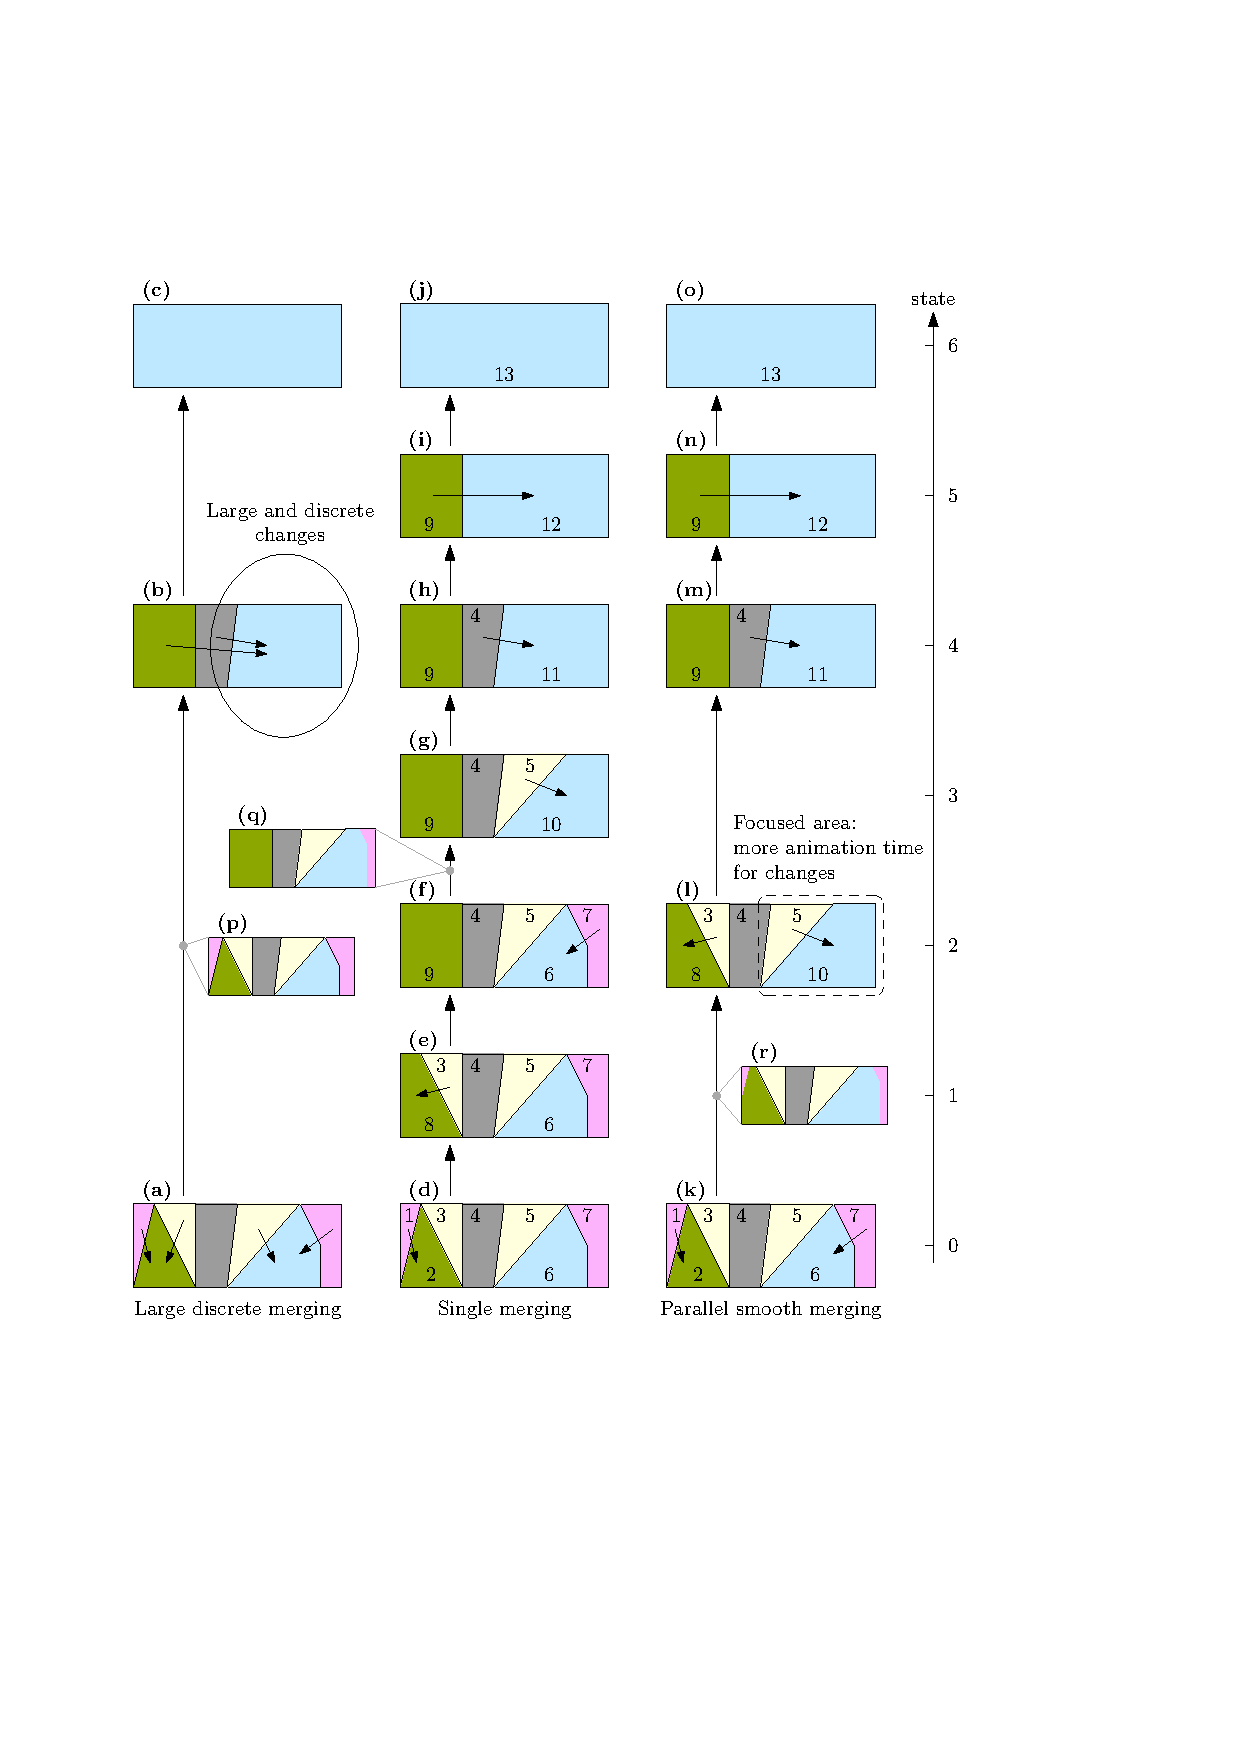
\includegraphics[page=1,scale=0.85]{intro}
\caption{A comparison of different scale-transition strategies.
Each arrow inside the subfigures indicates a merging operation.
The arrow in the right-hand side indicates the states of zooming out.
%
(a--c): All changes are processed in one go.
(d--j): All changes are sequenced one by one rapidly.
(k--o): Changes are grouped, resulting in more animation duration for every change.
%where smooth and parallel changes going on can be found in figure~(r);
%digital map with smooth and parallel generalization operations.
%
The numbers are the face IDs.
}
\label{fig:intro}
\end{figure*}



\begin{figure*}[htb]
\centering
\begin{subfigure}[t]{0.48\textwidth}
\centering
\includegraphics[page=4,width=0.7\linewidth]{methodology}
\caption{The SSC of the single merging of \figs\ref{fig:intro}d--j.}
\end{subfigure}
\hfill
\begin{subfigure}[t]{0.48\textwidth}
\centering
\includegraphics[page=5,width=0.7\linewidth]{methodology}
\caption{The SSC of the parallel merging of \figs\ref{fig:intro}k--o.}
\end{subfigure}
\caption{
In the left SSC, only one merging event is happening 
at a specific state ($z$-dimension), 
while in the right SSC multiple merging events may happen at the same state.
}
\label{fig:ssc}
\end{figure*}


We define an \emph{event} as a single generalization operation, 
such as merging an area into a neighbor.
Two areas are neighbors if they share a common boundary with length larger than 0
(sharing a point does not make the two areas neighbors).
For example, \fig\ref{fig:intro}e is obtained from 
\fig\ref{fig:intro}d by processing one merging event.
Similarly, \fig\ref{fig:intro}l is obtained from 
\fig\ref{fig:intro}k by processing two merging events.
We define a \emph{step} as 
a set of events happening at the same animation duration.
%For example, 
%\fig\ref{fig:intro}e is obtained from 
%\fig\ref{fig:intro}d by processing a step with one merging event.
%\fig\ref{fig:intro}l is obtained from 
%\fig\ref{fig:intro}k by processing a step with two merging events.
In our method, a step is completely processed 
before the next step takes place (all sequential).
We define a \emph{state} as the point when a step starts or finishes.
For example, there are seven states 
in the merging sequence of \figs\ref{fig:intro}d--j
and five states in the merging sequence of \figs\ref{fig:intro}k--o 
(\ie~states 0, 2, 4, 5, and 6).
Note that the value of a state is also 
the total number of events processed so far.

There are two benefits of paralleling merging operations.
First, parallelization avoids unnatural zooming.
Without parallelization,
sequentially processing generalization operations 
may result in no change at some locations in a zooming duration, 
which is unnatural \citep{vanOosterom2014Support}. 
Therefore, \citet{vanOosterom2014Support} 
suggested paralleling the generalization operations,
but no implementation, testing, or assessment of the idea was provided.
Second, parallelization brings smoother zooming.
Although the SSC allows to deliver a map at any scale,
only $16$ frames by default will be created to display in one second.
When showing an animation zooming, 
we set $16$ as the default value of frames per second (FPS).
This value is adequate to provide the visual continuity
\citep[\p24]{Read2000Film}.
If the merging operations happen sequentially instead of parallelly,
it is more likely that
the gap between two frames is larger than the gap between two states.
Then there is no animation of smooth merging at all.
For example, if the consecutive frames are 
\figs\ref{fig:intro}d, \ref{fig:intro}e, and \ref{fig:intro}f,
then users can only see discrete merging.
In contrast, if the consecutive frames are 
\figs\ref{fig:intro}k, \ref{fig:intro}r, and \ref{fig:intro}l,
then users can really see an ongoing expansion. 
The more merging operations we parallel, 
the smoother the expansion process seems.

%\textbf{one step 16 frames or one second 16 frames?}
%answer: one second 16 frames

When merging parallelly,
we require that 
the area objects involved in different merging events of the same step 
must not be neighbors, 
which makes the merging events independent from each other.
In this way, it is easy for us to maintain the topology of the map.
%Second, users can keep track of their area objects of interest more easily
%than merging several areas into a single one.
In order to realize the requirement,
we block the neighbors of the areas once we have found an event.
We show a greedy algorithm to find the parallel merging events for each step
in \sect\ref{sec:greedy_algo}.
Then, we integrate the events into the tGAP database tables
(\sect\ref{sec:integrate_tgap}),
followed by integrating the events into the SSC 
(\sect\ref{sec:integrate_ssc}).
In \sect\ref{sec:snap}, we show how to snap the zooming to valid states
to avoid half-way merging animation 
as stopping halfway will result in showing slivers at a static state.
In \sect\ref{sec:zooming_duration}, we define 
the animation duration of zooming from one state to another state.


\subsection{A greedy algorithm}
\label{sec:greedy_algo}

For each merging event, our greedy algorithm tries to 
merge the least important area into its most compatible neighbor.
%There are many ways of defining the most compatible neighbor.
%For example, \citet{Cheng2006} proposed three choices, i.e.,
%the neighbor has the largest size, 
%shares the longest boundary with the least important area,
%or has the closest class to the least important area. 
%\citet{Peng2017AStar} proposed that 
%the most compatible neighbor should have a close class
%to the least important area
%and the combination of the two areas should be compact;
%they defined the class distance based on a binary tree
%according to the codes of the classes.
We define the importance and the compatibility according to
%\citet{vanOosterom2005,vanPutten1998NewGAP}.
\citet{vanPutten1998NewGAP}.
That is, the importance of an area is the multiplication 
of its size and its class weight.
Currently, all the class weights are set to 1,
which leads to that the smallest area is the least important.
The compatibility value between a pair of areas is 
the multiplication of the common boundary's length and 
the class similarity of the two areas.
%\appx\ref{appx:create_tables} shows our implementation of
%computing the weight values and the class similarities.



\fig\ref{fig:greedy_framework} shows the flowchart of our greedy algorithm.
The process starts with state~$s=0$ and a detailed map of area objects, $M_0$.
Expression~$|M_s|$ denotes the number of area objects of the map at state~$s$.
Parallel parameter~$r_\mathrm{parallel}$ specifies 
the proportion (\ie~percentage, when multiplied by~$100$) of the number
of the area objects that
we expect to merge parallelly,
where~$r_\mathrm{parallel} \in [0,1]$.
Variable~$n_\mathrm{target}$ denotes the number of area objects
that we expect to merge in a step.
%As a value of percentage, 
%$r_\mathrm{parallel}$ is in the range from~$0\%$ to~$100\%$,
%which means~$r_\mathrm{parallel} \in [0,1]$.
%If there is more than one area ($|M_s|>1$),
%then we start finding merging events.
%We first compute the number of areas that we expect to merge by
%\begin{equation}
%\label{eq:n_target}
%n_\mathrm{target} =
%\lceil r_\mathrm{parallel} \cdot |M_s| \rceil,
%\end{equation}
%where the ceiling function guarantees~$n_\mathrm{target}\ge 1$.
%That is to say, we find at least one event for each step.
However,
we cannot always find~$n_\mathrm{target}$ events
because some areas may be blocked as explained before
(also see \fig\ref{fig:blocked_polygons}).
Therefore, we use variable~$n_\mathrm{event}$
to represent the number of events that actually happened within the step. 
In the algorithm, an area is \emph{free} if 
it is not involved in an event and is not blocked.
\fig\ref{fig:blocked_polygons} shows an example of blocking
the surrounding neighbors of~$a_\mathrm{least}$ and~$a_\mathrm{nbr}$.
Note that the gray area in \fig\ref{fig:blocked_polygons}a is not blocked
because it is not considered a neighbor of the green area
(sharing a point does not make the two areas neighbors). 




\begin{figure*}[tb]
\centering
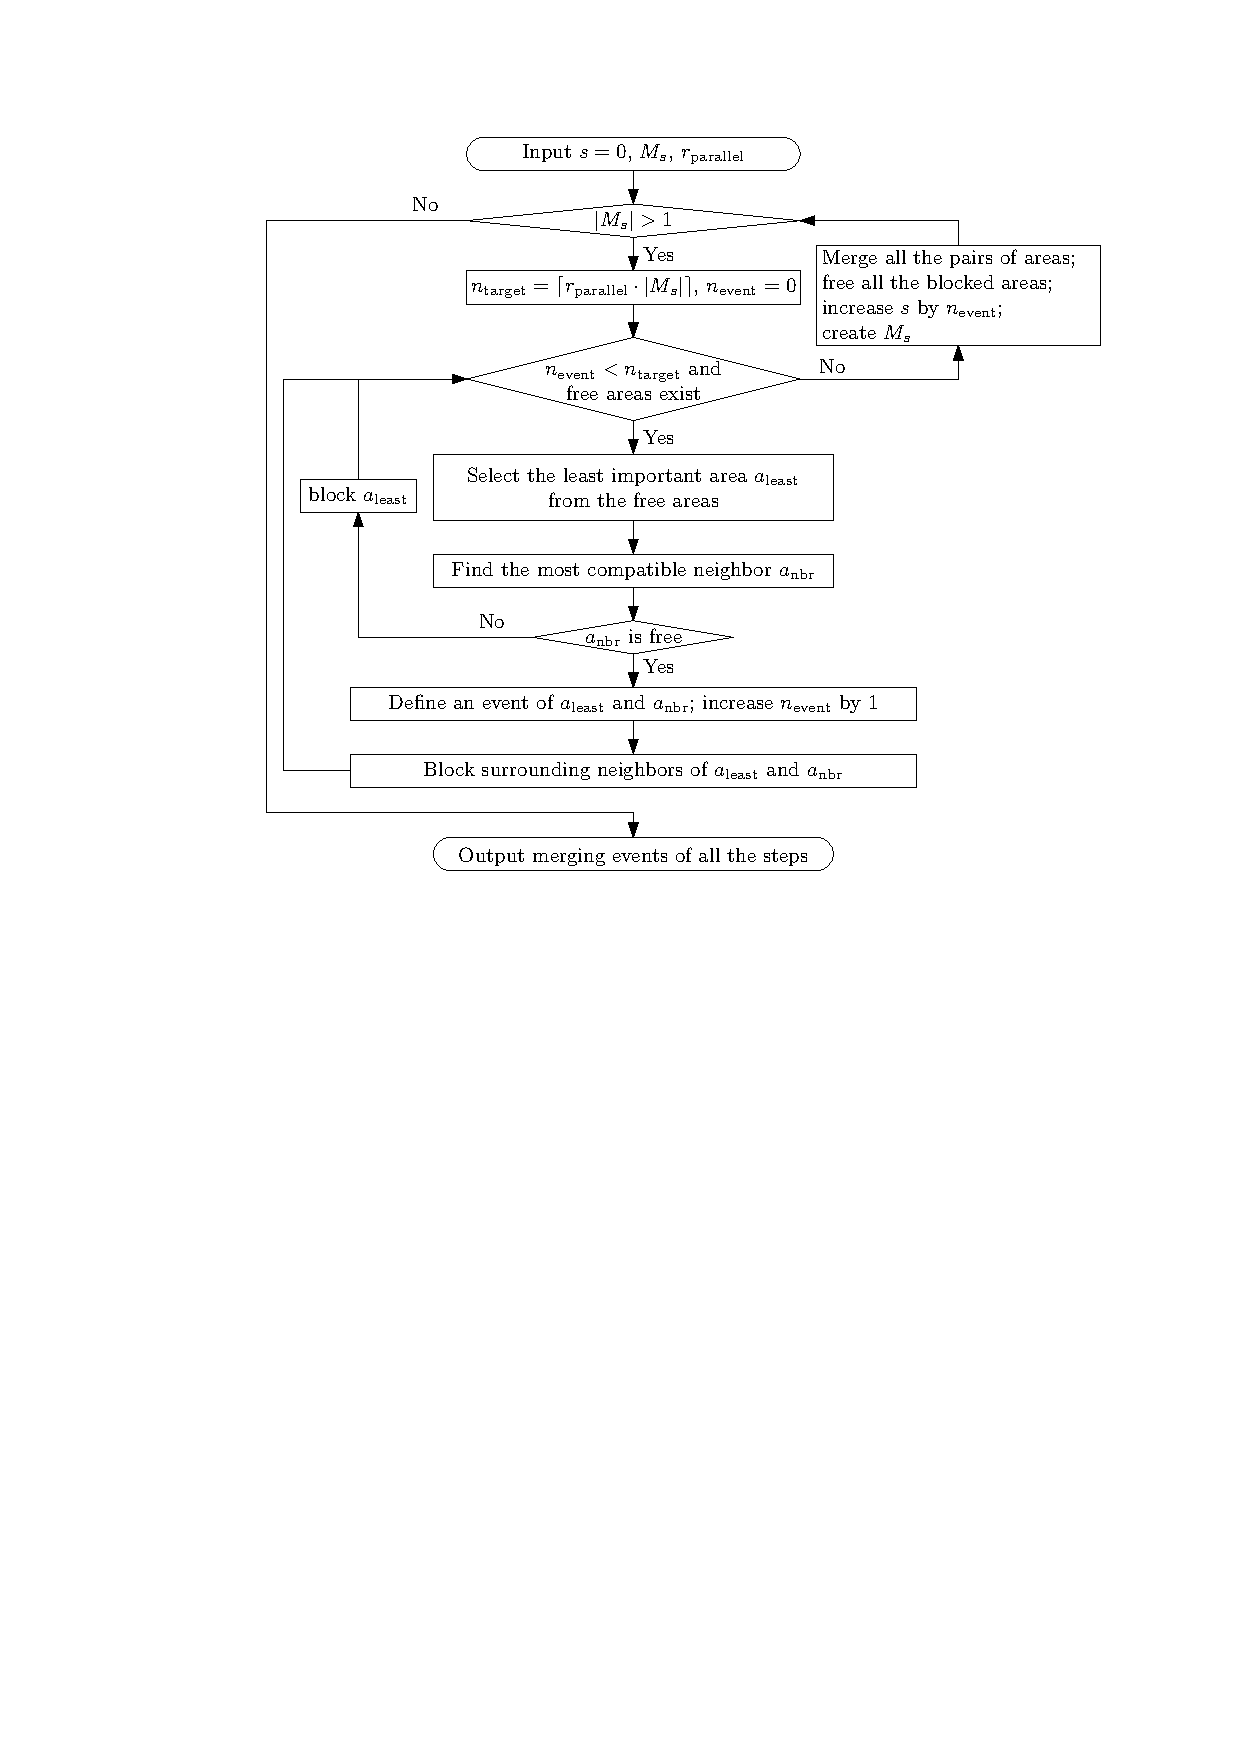
\includegraphics[page=1,scale=0.85]{methodology}
\caption{The flowchart of our greedy algorithm
    to find the merging events for all the steps.
}
\label{fig:greedy_framework}
\end{figure*}


\begin{figure*}[tb]
\centering
\includegraphics[page=2,scale=0.85]{methodology}
\caption{The process of finding parallel merging events for a step, 
    where parallel parameter $r_\mathrm{parallel} = 0.3$.
    (a) From all the free areas,
	the least important one is selected to merge into
	its most compatible neighbor.
	Then the surrounding areas are blocked (marked by the crosses).
	(b) Next, the least important area from the remaining free areas
	is selected to merge with the most compatible neighbor,
	and the surrounding areas are also blocked.
}
\label{fig:blocked_polygons}
\end{figure*}

%If we have not found $n_\mathrm{target}$ events 
%($n_\mathrm{event} < n_\mathrm{target}$)
%and there are still free areas,
%then we go on looking for merging events.
%We select the least important area~$a_\mathrm{least}$
%from the free areas.
%An area is \emph{free} if 
%it is not involved in an event and is not blocked.
%We also find~$a_\mathrm{least}$'s 
%most compatible neighbor~$a_\mathrm{nbr}$.
%If area~$a_\mathrm{nbr}$ is also free, 
%we define an event of areas~$a_\mathrm{least}$ and~$a_\mathrm{nbr}$.
%Then, we increase the number of events, $n_\mathrm{event}$, by 1.
%We block the surrounding neighbors of~$a_\mathrm{least}$ and~$a_\mathrm{nbr}$
%(see \fig\ref{fig:blocked_polygons}a).
%Note that the area shares only a vertex 
%with the least important area is not blocked.
%If area~$a_\mathrm{nbr}$ is not free,
%then it must be blocked because of the previously found events.
%In this case, we block $a_\mathrm{least}$ for now
%so that areas~$a_\mathrm{least}$ and~$a_\mathrm{nbr}$ 
%may merge in the next step.
%Then, we continue to find more merging events and to block more areas
%(see \fig\ref{fig:blocked_polygons}b).

%If we have found~$n_\mathrm{target}$ events 
%or there is no free area anymore,
%then finding merging events of the step finishes.
%We parallelly merge all the pairs of areas of the found events
%to generate new areas,
%free all the blocked areas,
%increase state~$s$ by value~$n_\mathrm{event}$,
%and create map~$M_s$ based on the new areas and the freed areas.
%Then, finding merging events for the next step starts.
%This iteration of finding completes 
%until there is only one area left on the map ($|M_s|=1$).
Finally, the merging events will be stored 
as records in tGAP database tables
(see \fig\ref{fig:uml_tgap}).
\figs\ref{fig:intro}k--o show a sequence of four merging steps
obtained by our greedy algorithm,
where parallel parameter~$r_\mathrm{parallel}$ is set to~$0.3$
(Note that this is an extremely high value, 
just used to explain the principle in an artificial simple example).



\begin{figure}[tb]
\centering
\includegraphics[page=3,scale=0.83]{methodology}
\caption{The UML diagram of the classes stored in tGAP database tables.
This diagram is a slightly improved version of \citet[\p159]{Meijers2011Thesis}.
In the face table, property \emph{pip\_geometry} 
stores a point (usually the center) in the face (polygon).
%The geometry of a face can be obtained by calling function \emph{getGeometry()}.
%We do not store the face geometry because we want to avoid redundancy,
%as the edges already stores the sequences of points.
}
\label{fig:uml_tgap}
\end{figure}


\subsection{Integrating the parallel events into the tGAP database tables}
\label{sec:integrate_tgap}

\citet[\p159]{Meijers2011Thesis} designed three tables 
to record the information of
faces, edges, and face hierarchies, 
which together form a tGAP
(also see \fig\ref{fig:uml_tgap}).
%For example, the face table contains columns \emph{face\_id}, 
%\emph{imp\_low}, \emph{imp\_high}, \emph{imp\_own},
%\emph{feature\_class}, \emph{area}, and \emph{mbr\_geometry}.
We add columns \emph{state\_low} ($s_\mathrm{low}$) 
and \emph{state\_high} ($s_\mathrm{high}$) into the table 
so that it is easy to see when a face should appear or disappear 
(see \tbls\ref{tbl:face_tgap}a and~\ref{tbl:face_tgap}b,
where all other columns, except face\_id, are hidden).
For zooming out,
when the slicing plane arrives at the low state of a face,
the face appears because of the merging of two faces.
When the slicing arrives at the high state,
the face should merge with another area.
Comparing between the tables of single merging 
and parallel merging,
we observed some differences of the values.
For example, the $s_\mathrm{high}$ values of faces~1 and~2 
are changed from~$1$ to~$2$
(see \tbl\ref{tbl:face_tgap}).
Also, the $s_\mathrm{low}$ value of face~8 is changed from~1 to~2
(see \tbl\ref{tbl:face_tgap}).
Note that the face ids are defined in \fig\ref{fig:intro}.
Similarly, the columns and records of 
both the edge table and the face-hierarchy table 
will be changed accordingly.


\begin{table*}[tb]
\caption{Some columns of the face tables. 
    Columns~$s_\mathrm{low}$, $s_\mathrm{merge}$, 
    and~$s_\mathrm{high}$ show the states 
    when the faces appear, when the faces start to disappear, and
    when the faces completely disappear.    
    In table~(b), the different values from table~(a) are underlined.
    Column~$s_\mathrm{merge}$ is not really stored in the database.
    We show the column so that it is easy to see the differences 
    between the $s_\mathrm{low}$ values and the $s_\mathrm{merge}$ values.
    }
\label{tbl:face_tgap}
\begin{subtable}{0.48\textwidth}
\caption{The face table of the single merging 
    shown in \figs\ref{fig:intro}d--j.}
\centering
\begin{tabular}{cccc}
\toprule
$f_\mathrm{id}$& $s_\mathrm{low}$    & $s_\mathrm{merge}$ & $s_\mathrm{high}$ \\ \midrule
1       &     0         &     0         &     1       \\
2       &     0         &     0         &     1       \\
3       &     0         &     1         &     2       \\ 
4       &     0         &     4         &     5       \\
5       &     0         &     3         &     4       \\
6       &     0         &     2         &     3       \\         
7       &     0         &     2         &     3       \\
8       &     1         &     1         &     2       \\
9       &     2         &     5         &     6       \\         
10      &     3         &     3         &     4       \\
11      &     4         &     4         &     5       \\ 
12      &     5         &     5         &     6       \\ 
13      &     6         &    ---        &    ---      \\
\bottomrule
\end{tabular}
\end{subtable}
%
\hfill
%
\begin{subtable}{0.48\textwidth}
\caption{The face table of the parallel merging 
    shown in \figs\ref{fig:intro}k--o.}
\centering
\begin{tabular}{cccc} %\underbar{2}
\toprule
$f_\mathrm{id}$ & $s_\mathrm{low}$   & $s_\mathrm{merge}$ & $s_\mathrm{high}$ \\ \midrule
1       &     0         &     0         &\underbar{2} \\
2       &     0         &     0         &\underbar{2} \\
3       &     0         & \underbar{2}  &\underbar{4} \\ 
4       &     0         &     4         &     5       \\
5       &     0         & \underbar{2}  &     4       \\
6       &     0         & \underbar{0}  &\underbar{2} \\         
7       &     0         & \underbar{0}  &\underbar{2} \\
8       & \underbar{2}  & \underbar{2}  &\underbar{4} \\
9       &     2         &     5         &\underbar{6} \\         
10      & \underbar{4}  & \underbar{2}  &\underbar{4} \\
11      &     4         &     4         &     5       \\ 
12      &     5         &     5         &     6       \\ 
13      &     6         &    ---        &    ---      \\
\bottomrule
\end{tabular}
\end{subtable}
\end{table*}


\subsection{Integrating the parallel events into the SSC}
\label{sec:integrate_ssc}

Recall that we merge a pair of areas by expanding 
the more important one over the less important one.
The Eater of \citet{Suba2014Merge} is used to 
triangulate the less important area and to tilt the triangles.
Then the tilted triangles are integrated into the SSC
(see \fig\ref{fig:ssc})
so that we can slice the SSC to achieve smooth merging.
For the case of single merging,
if a pair of areas have state-high value~$s_\mathrm{high}$,
then the merging animation 
always starts at state~$s_\mathrm{merge}=s_\mathrm{high}-1$
(see \tbl\ref{tbl:face_tgap}a).
The less important area completely disappears
at state~$s_\mathrm{high}$.
In the face table, a row will be added to record the new area, 
and its $s_\mathrm{low}$ value will be the previous~$s_\mathrm{high}$ value.
The new area takes the combined place of the pair of areas.
Take \fig\ref{fig:intro} as an example, 
area~1 is merged into area~2 (\figs\ref{fig:intro}d), 
and area~8 is generated to take the combined place (\figs\ref{fig:intro}e).
The tilted triangle is the one that spans 
from~$z= 0$ to~$z=100$ (\ie~from state~0 to state~1)
in \fig\ref{fig:ssc}a.
In \tbl\ref{tbl:face_tgap}a, 
the~$s_\mathrm{low}$ value of area~8 is 1,
which is the~$s_\mathrm{high}$ values of areas~1 and~2.
%Note that the state\_low values of the two areas do not matter 
%because those values respectively indicate the states that
%the two areas appear;
%those values can be much smaller 
%than value~$s_\mathrm{high}-1$.

For the case of parallel merging,
if a step consists of~$n_\mathrm{event}$ events and 
the step finishes at state~$s_\mathrm{high}$, then the step starts 
at state~$s_\mathrm{merge}=s_\mathrm{high} - n_\mathrm{event}$.
The reason is that if the~$n_\mathrm{event}$ events 
would happen sequentially (\ie~single merging),
then they would take place 
from state~$s_\mathrm{high} - n_\mathrm{event}$ to state~$s_\mathrm{high}$.
When all the events take place parallelly in the same step, 
each of the events can share its merging duration.
%there is a less important area in each of the parallel events of a merging step.
%If the number of parallel events is~$n_\mathrm{event}$,
%then there are~$2n_\mathrm{event}$ areas 
%with the same state\_high value, say,~$s_\mathrm{high}$
%because each merging event involves two areas.
%The merging animations of all the parallel events
%start at state~$s_\mathrm{merge}=s_\mathrm{high} - n_\mathrm{event}$
%and finishes at state~$s_\mathrm{high}$.
%By definition, the parallel events of a merging step 
%happen during the same animation time.
%In other words, the areas involved in those parallel events have 
%the same state\_merge value ($s_\mathrm{merge}$) and 
%the same state\_high value ($s_\mathrm{high}$).
%The reverse is also true.
%If some areas have the same state\_high value,
%then those areas happen during the same animation time 
%(involved in the parallel events of the same step).
%The reason is that, according to our requirement,
%a step can start only when the previous step stops.
%Thus, the merging events finishing at the same state cannot from different steps.
%of these areas 
%will finish at state~$s_\mathrm{high}$,
%and no merging event will start earlier or later than state~$s_\mathrm{merge}$
%because we required that the next step starts only when a step stops.
%Given the fact that the merging duration for zooming 
%between states~$s_\mathrm{merge}$ and~$s_\mathrm{high}$ is fixed,
As a result,
each of the parallel events has more time to take place
than the events would happen sequentially.
In other words, for a merging step,
each of the events has more time to take place 
if there are more parallel events.

%In order to build the SSC for parallel merging,
%we need the~$s_\mathrm{merge}$ value for each of the merging steps
%so that we know from which state 
%the triangles of the less important areas should be tilted.
%%A simple way is to add a column, say, $s_\mathrm{merge}$
%%into the face table during generating the tGAP, 
%%as done in \tbl\ref{tbl:face_tgap}.
%%Then, the states of starting merging can be recorded into the column.
%%However, we would like to avoid unnecessary columns to save storage.
%%Therefore, we compute~$s_\mathrm{merge}$ values 
%We compute~$s_\mathrm{merge}$ values 
%based on the~$s_\mathrm{high}$ values
%on the fly when building the SSC.
%As an event involves two areas,
%the number of events finishing at state~$s_\mathrm{high}$ can be calculated by
%\begin{equation*}
%\label{eq:n_event_state}
%n_\mathrm{event} (s_\mathrm{high}) = 
%\frac{\sum\limits_{s \in S_\mathrm{high}} [s=s_\mathrm{high}]}{2},
%\end{equation*}
%where notation~$S_\mathrm{high}$ denotes the set of values
%recorded in column~$s_\mathrm{high}$ of the face table
%(\eg~\tbl\ref{tbl:face_tgap}b).
%Expression~$[s=s_\mathrm{high}]$ returns~$1$ if the two values are equal 
%and returns~$0$ otherwise.
%As illustrated before, the state at which the parallel merging starts 
%can be computed by
%\begin{equation*}
%\label{eq:s_merge_state}
%s_\mathrm{merge} (s_\mathrm{high}) = s_\mathrm{high} - n_\mathrm{event} (s_\mathrm{high}).
%\end{equation*}
%Based on the values of \tbl\ref{tbl:face_tgap}b,
%we are able to build the SSC of \fig\ref{fig:ssc}b.


%Take the case of \tbl\ref{tbl:face_tgap}b for example,
%we have~$S_\mathrm{high} = \{2, 2, 4, 5, 4, 2, 2, 4, 6, 4, 5, 6\}$, 
%$n_\mathrm{event} (4) = 2$, and~$s_\mathrm{merge} (4) = 2$.
%Therefore, there are two merging events finishing at state~$4$,
%\ie~event of merging area 3 into area~8 and 
%event of merging area~5 into area~10 
%(also see \figs\ref{fig:intro}l and~\ref{fig:intro}m).
%The merging animation takes place from state~$2$ to state~$4$.
%This merging can be also observed from 
%the two tilted triangles spanning from~$z = 200$ to~$z = 400$ 
%in \fig\ref{fig:ssc}b.
%In merging sequence of \figs\ref{fig:intro}d--j, 
%the animation of merging area~3 into area~8 
%takes place from state~$1$ to state~$2$
%(also see the tilted triangle spanning from~$z = 100$ to~$z = 200$ 
%in \fig\ref{fig:ssc}a), and 
%the animation of merging area~5 into area~10
%takes place from state~$3$ to state~$4$
%(also see the tilted triangle spanning from~$z = 300$ to~$z = 400$ 
%in \fig\ref{fig:ssc}a).
%As a result, the animation duration of merging area~3 into area~8 of 
%sequence \figs\ref{fig:intro}k--o
%is almost twice as that of sequence \figs\ref{fig:intro}d--j.
%We say \emph{almost} because the animation duration is also dependent on 
%the current state of the map
%(see \sect\ref{sec:zooming_duration}).


\subsection{Snapping to a valid state}
\label{sec:snap}

For a zooming action based on the SSC, 
we always snap the map to a valid state.
In this way, we can avoid that a merging operation stops half-way,
and users will not see transition artifacts (such as slivers).
Take the sequence of \fig\ref{fig:intro}k--o for example, 
the merging animation should stop at 
either \ref{fig:intro}k or \ref{fig:intro}l,
but not at \ref{fig:intro}r.
Note that some states are not valid because of the parallel events.
For example, state~$1$ is not valid 
in the sequence of \fig\ref{fig:intro}k--o,
where the list of valid states 
is~$S_\mathrm{valid} = [0, 2, 4, 5, 6]$.
In order to snap to one of the valid states after a zooming operation,
we have to communicate them to the client side. 
There are multiple options. 
The most simple one assumes that, 
during the creation of the parallel SSC, 
we can always perform 
the~$n_\mathrm{target}$ number of events in all steps. 
In that case, we just have to communicate 
the number of areas and the ratio~$r_\mathrm{parallel}$. 
In case of high value ratios (\eg~$r_\mathrm{parallel} > 0.01$), 
this assumption may be incorrect. 
We then have to communicate the valid states by sending them explicitly. 
Because this list may get rather large,
we only send exceptions.
%\appx\ref{appx:communicate_valid_states} shows the details of the technique.
%As a result, the list of valid states~$S_\mathrm{valid}$ is sent to the client side.


According to how much a user has zoomed,
the target scale (\ie $1:S_\mathrm{t}$) can be computed.
%According to \citet{Huang2016Webmap},
%the number of merging events that should be processed can be computed by
\citet{Huang2016Webmap} suggested that 
the average density of the original map should be preserved 
for a smaller-scale map.
Their suggestion is based on the assumption that 
the area density of the base map is well designed, which is reasonable.
We use variable~$A_\mathrm{real}$ to denote the total areal size in reality
of all the area objects .
Then, the size on screen at scale~$1:S_\mathrm{t}$ 
is~$A_\mathrm{real} \big/ S^2_\mathrm{t}$.
In order to keep the density, we require
\begin{equation}
\label{eq:equal_density}
\frac{N_\mathrm{b}}{A_\mathrm{real} \big/ S^2_\mathrm{b}} =
\frac{N_\mathrm{b}-E_\mathrm{t}}{A_\mathrm{real} \big/ S^2_\mathrm{t}},
\end{equation}
where parameter~$N_\mathrm{b} = |M_0|$ 
is the number of areas on the base map,
parameter~$S_\mathrm{b}$ is the scale denominator of the base map,
and variable~$E_\mathrm{t}$ is the total number of events 
happening from the base map to the map at scale~$1:S_\mathrm{t}$
(in this case, an event is that an area is merged into another one).
\eq\ref{eq:equal_density} yields
\begin{equation}
\label{eq:E_t}
E_\mathrm{t} = N_\mathrm{b} \left(1-\frac{S^2_\mathrm{b}}{S^2_\mathrm{t}}\right),
\end{equation}
In our example regarding to list of valid states~$\mathrm{S_\mathrm{valid}}$,
if event number~$E_\mathrm{t} \le 0$, the base map should be presented;
if $E_\mathrm{t} \ge 6$, 
%(\ie~the last value of list~$L_\mathrm{event}$),
the map with the final single area should be presented.
Otherwise, if $0<E_\mathrm{t} < 6$, we snap event number~$E_\mathrm{t}$ 
to the closest value (measured in events) of list~$S_\mathrm{valid}$.
The snapped number of events 
is denoted by $E_\mathrm{t,snap}$.
The scale denominator corresponding to event number~$E_\mathrm{t,snap}$
can be computed by 
\begin{equation}
\label{eq:S_t_snap}
S_\mathrm{t,snap} = S_\mathrm{b} \sqrt{\frac{N_\mathrm{b}}{N_\mathrm{b}-E_\mathrm{t,snap}}}.
\end{equation}
where this equation is an inverse function of \eq\ref{eq:E_t}.
At the end of the zooming action, 
the map will snap to state~$s_\mathrm{t,snap}$
at scale~$1:S_\mathrm{t,snap}$.
Note that state~$s_\mathrm{t,snap}$ always has 
the same value as event number~$E_\mathrm{t,snap}$.



%\subsection{Line simplification (smoothly moving vertices for the SSC)}


\subsection{Animation duration of a step}
\label{sec:zooming_duration}

When users are zooming from a scale to another scale,
some steps take place to change the map from a state to another one.
We define the \emph{zooming duration} as the amount of 
animation time that the map reacts to one scroll of the mouse wheel.
The zooming duration often is the sum of 
the \emph{animation durations} of several merging steps.
The animation duration of each event depends on 
the number of events between the two states,
the \emph{zooming factor} of the scale, and 
the \emph{zooming duration}.
On the one hand, the animation duration should not be too short 
as then the animation will be too fast. 
On the other hand, if the animation takes too long, 
the map will not be interactive, and users will be ``frustrated''.
\citet[][\sect4.3]{Meijers2020Web} 
have introduced the zooming factor and the zooming duration.
They allowed users to set the two parameters,
which is also the case in this paper.
%(see \fig\ref{fig:interaction_settings}).
Because of the page limit, 
we skip the deductions and show some conclusions as following. 
The animation duration of a set of events happening sequentially is
\begin{equation*}
\label{eq:t_single}
t_\mathrm{single} = \frac{t_\mathrm{zoom}}{N_\mathrm{event}},
\end{equation*}
where~$t_\mathrm{zoom}$ is the zooming duration, 
and $N_\mathrm{event}$ is the number of events
happening in one scroll of the mouse wheel.
The animation duration of a set of events happening parallelly is
\begin{equation*}
\label{eq:t_parallel}
t_\mathrm{parallel} = \frac{t_\mathrm{zoom}}{n_\mathrm{step}},
\end{equation*}
where~$n_\mathrm{step}$ is the number of steps
happening in one scroll of the mouse wheel.
%\begin{equation*}
%\label{eq:t_compare}
%t_\mathrm{parallel} = t_\mathrm{single}  \frac{N_\mathrm{event}}{n_\mathrm{step}},
%\end{equation*}
%where~$N_\mathrm{event}$ and~$n_\mathrm{step}$ are respectively
%the number of events and the number of steps
%happening in one scroll of the mouse wheel.
%Variables $t_\mathrm{single}$ and $t_\mathrm{parallel}$ are respectively
%the animation durations of the events happening singly and parallelly.
As~$N_\mathrm{event}$ is larger than or equal to~$n_\mathrm{step}$,
we have $t_\mathrm{parallel} \ge t_\mathrm{single}$.
%$t_\mathrm{parallel}$ is larger than or equal to~$t_\mathrm{single}$.




%This section formalizes the relationship of the animation duration,
%the zooming duration, the zooming factor, and the number of events.
%
%In a zooming duration, there can be many merging steps,
%no matter single merging or parallel merging.
%The following calculation is based on the setting that
%a zooming duration is divided equally by its merging steps
%(\citet[][\sect6.7]{Suba2017Thesis} showed some other possible settings).
%In other words,
%the steps happen sequentially and take the same amount of animation duration.
%Note that the steps from different zooming durations 
%may have different animation durations.
%%In the following calculation, 
%%we assume that we can always find the target number 
%%(see \eq\ref{eq:n_target})
%%of events for all the steps.
%%If there are exceptions, 
%%then the following calculation should be adjusted accordingly.
%
%%\begin{figure}[tb]
%%\centering
%%\includegraphics[page=6,scale=0.6]{methodology}
%%\caption{Our panel of settings. 
%%Among others, one can set how much to zoom when scrolling the mouse wheel 
%%and set the zooming duration.}
%%\label{fig:interaction_settings}
%%\end{figure}
%
%
%Let~$f_\mathrm{zoom}$ be the zooming factor, and 
%let~$t_\mathrm{zoom}$ be the zooming duration.
%Let~$1:S_\mathrm{t,snap}$ be the snapped scale before the zooming operation, and 
%let~$1:S_\mathrm{o}$ be the zoomed out scale (not snapped yet).
%For zooming out, we define the relationship 
%between the two scale denominators as
%\begin{equation}
%\label{eq:S_o}
%S_\mathrm{o} = S_\mathrm{t,snap} (1 + f_\mathrm{zoom}).
%\end{equation}
%For scale~$1:S_\mathrm{o}$, we compute the number of events
%that should be processed from the base map by
%\begin{equation*}
%\label{eq:E_o}
%E_\mathrm{o} = N_\mathrm{b} \left(1-\frac{S^2_\mathrm{b}}{S^2_\mathrm{o}}\right),
%\end{equation*}
%which is according to \eq\ref{eq:E_t}.
%As the value of~$E_\mathrm{o}$ may be not an integer, 
%we snap it to a valid state
%(see \sect\ref{sec:snap}),
%and we have a snapped value~$E_\mathrm{o,snap}$.
%Then, we compute scale denominator~$S_\mathrm{o,snap}$
%by \eq\ref{eq:S_t_snap}.
%According to \eq\ref{eq:E_t}, we have merged~$E_\mathrm{t,snap}$ areas 
%when arriving at scale~$1:S_\mathrm{t,snap}$.
%The event number of zooming out
%from scale~$1:S_\mathrm{t,snap}$ to scale~$1:S_\mathrm{o,snap}$ is
%%$
%\begin{equation*}
%\label{eq:N_event}
%N_\mathrm{event} = 
%E_\mathrm{o,snap} - E_\mathrm{t,snap}.
%\end{equation*}
%%$
%%Accordingly, we can compute scale denominator~$S_\mathrm{o,snap}$
%%by \eq\ref{eq:S_t_snap}
%Recall that zooming duration~$t_\mathrm{zoom}$ is for zooming 
%from scale~$1:S_\mathrm{t,snap}$ to scale~$1:S_\mathrm{o}$.
%As the map is actually zooming to~$1:S_\mathrm{o,snap}$,
%we adjust the zooming duration to
%\begin{equation*}
%\label{eq:E_i}
%t_\mathrm{snap}= t_\mathrm{zoom} 
%%\frac{n_\mathrm{event}}
%\frac{N_\mathrm{event}}
%{E_\mathrm{o} - E_\mathrm{t,snap}}.
%\end{equation*}
%%\begin{equation}
%%\label{eq:n_event}
%%n_\mathrm{event} 
%%= E_\mathrm{o} - E_\mathrm{t,snap}
%%= N_\mathrm{b} S^2_\mathrm{b} \left(\frac{1}{S^2_\mathrm{t,snap}} - \frac{1}{S^2_\mathrm{o}}\right).
%%\end{equation}
%That is to say, the~$E_\mathrm{o,snap} - E_\mathrm{t,snap}$ events will happen 
%in time duration~$t_\mathrm{snap}$.
%If the events happen sequentially (each step consists of a single event), 
%then the animation duration of each event is
%\begin{equation}
%\label{eq:t_single}
%t_\mathrm{single}   = \frac{t_\mathrm{snap}}{N_\mathrm{event}} 
%                    = \frac{t_\mathrm{zoom}}{E_\mathrm{o} - E_\mathrm{t,snap}}.
%\end{equation}
%
%If we parallel these events, 
%then we will have fewer steps and 
%each event has more time to take place.
%Let~$n_\mathrm{step}$ be the number of steps in a zooming duration.
%If we are lucky enough so that
%expression~$r_\mathrm{parallel} \cdot |M_s|$ of \eq\ref{eq:n_target}
%always returns an integer, 
%then we do not need the ceiling function of \eq\ref{eq:n_target}
%(if we are not that lucky, the value of~$n_\mathrm{step}$ will be slightly different).
%We have 
%\begin{equation*}
%%\label{eq:n_event}
%N_\mathrm{t,snap} (1-r_\mathrm{parallel})^{n_\mathrm{step}} = N_\mathrm{o,snap},
%\end{equation*}
%where~$N_\mathrm{t,snap} = N_\mathrm{b}- E_\mathrm{t,snap}$ 
%is the number of areas at scale~$1:S_\mathrm{t,snap}$,
%and~$N_\mathrm{o,snap} = N_\mathrm{b}- E_\mathrm{o,snap}$
%is the number of areas at scale~$1:S_\mathrm{o,snap}$.
%Then, the number of steps can be computed by
%\begin{equation*}
%%\label{eq:n_event}
%n_\mathrm{step} = \log_{1-r_\mathrm{parallel}} 
%    \frac{N_\mathrm{o,snap}}{N_\mathrm{t,snap}}.
%\end{equation*}
%Because the steps happen sequentially,
%each of the steps in the zooming duration has
%animation duration
%\begin{equation}
%\label{eq:t_parallel}
%t_\mathrm{parallel} = \frac{t_\mathrm{snap}}{n_\mathrm{step}},
%\end{equation}
%which is also the animation duration of each of the parallel events.
%Putting \eqs\ref{eq:t_single} and~\ref{eq:t_parallel} together,
%we have
%\begin{equation*}
%\label{eq:t_compare}
%t_\mathrm{parallel} = t_\mathrm{single}  \frac{N_\mathrm{event}}{n_\mathrm{step}}.
%\end{equation*}
%As~$N_\mathrm{event}$ is larger than or equal to~$n_\mathrm{step}$,
%$t_\mathrm{parallel}$ is also larger than or equal to~$t_\mathrm{single}$.
%
%
%When we zoom in back from scale~$S_\mathrm{o,snap}$ to scale~$S_\mathrm{t}$, 
%we have
%\begin{equation*}
%\label{eq:S_i}
%S_\mathrm{t} = \frac{S_\mathrm{o,snap}}{(1 + f_\mathrm{zoom})},
%\end{equation*}
%which is the inverse function of \eq\ref{eq:S_o}.
%We will be able to snap to scale~$1:S_\mathrm{t,snap}$.
%We will use the same animation duration and 
%process the same number of events and steps as we zoomed out.
%The difference from zooming out is that, instead of merging, 
%areas will bubble up.


%\bigskip
%\bigskip
%\bigskip
%\bigskip
%
%
%The number of remaining areas can be computed by
%\begin{equation}
%\label{eq:N_t}
%N_\mathrm{t,snap} 
%= N_\mathrm{b} - E_\mathrm{t,snap}
%= N_\mathrm{b} \frac{S^2_\mathrm{b}}{S^2_\mathrm{t,snap}}.
%\end{equation}
%Similarly, the number of areas at scale~$1:S_\mathrm{o}$ is 
%\begin{equation}
%\label{eq:N_o}
%N_\mathrm{o} 
%= N_\mathrm{b} \frac{S^2_\mathrm{b}}{S^2_\mathrm{o}}.
%\end{equation}
%
%Let~$1:S_\mathrm{o,snap}$ be the snapped scale of scale~$1:S_\mathrm{o}$.
%Similar to \eq\ref{eq:N_t}, the number of areas at scale~$1:S_\mathrm{o,snap}$ is
%\begin{equation}
%\label{eq:N_o_snap}
%N_\mathrm{o,snap} 
%= N_\mathrm{b} - E_\mathrm{t,snap}
%= N_\mathrm{b} \frac{S^2_\mathrm{b}}{S^2_\mathrm{o,snap}}.
%\end{equation}
%The number of events 
%from scale~$1:S_\mathrm{t,snap}$ to scale~$1:S_\mathrm{o,snap}$ is
%
%
%
%In \eq\ref{eq:n_event}, if we replace scale denominator~$S_\mathrm{o}$ by~$S_\mathrm{snap}$,
%then we obtain the event number, $n_\mathrm{snap}$, 
%to arrive the snapped scale (\ie~existing state), where
%\begin{equation}
%\label{eq:n_snap}
%n_\mathrm{snap} 
%= E_\mathrm{snap} - E_\mathrm{t}
%= N_\mathrm{b} S^2_\mathrm{b} \left(\frac{1}{S^2_\mathrm{t}} - \frac{1}{S^2_\mathrm{snap}}\right).
%\end{equation}
%
%
%We define the time duration for processing the $n_\mathrm{snap}$ events as


\section{Case study}
\label{sec:case_study}





%
\fig\ref{fig:data} shows the topographical map of this case study.
In each step, we want to parallelly merge some proportion of the areas.
We tried three cases: 0.1\%, 1\%, and 10\%.
The three versions of map can be browsed online.\footnote{%
All of our web maps can be found at
\url{https://pengdlzn.github.io/webmaps/2020/10/merge/}.}
As no paper has recommended values for 
the zooming factor or the zooming duration,
we respectively set the default values to $1$ and $1\,$s, 
which performed well according to our experience.
\fig\ref{fig:web_map} shows an example of our web map when 
parallel parameter~$r_\mathrm{parallel}=0.01$.
When zooming on our web maps with different parallel parameters,
we observed that the impressions of the maps 
based on single merging\footnote{%
See the web map at
\url{https://pengdlzn.github.io/webmaps/2020/10/merge/top10nl-single-merging.html}.} 
and based on parallel merging with parameter~$r_\mathrm{parallel}= 0.001$ 
are almost the same.
The reason is that the smooth merging happens too fast,
and we cannot really see the merging animation.
We get the feeling of smooth merging when~$r_\mathrm{parallel}= 0.01$.
When~$r_\mathrm{parallel}= 0.1$, 
the smooth merging is even more clearly visible.
In order to show a better comparison of single merging 
and parallel merging,
we put two maps together (see \fig\ref{fig:comparison}),
where the parallel parameter is~$0.1$.\footnote{%
See the map of comparison at
\url{https://pengdlzn.github.io/webmaps/2020/10/merge/top10nl-0.1-comparer.html}.}  




\begin{figure}[tb]
\centering
%trim = l b r t
%make b = l + r so that the map is a square
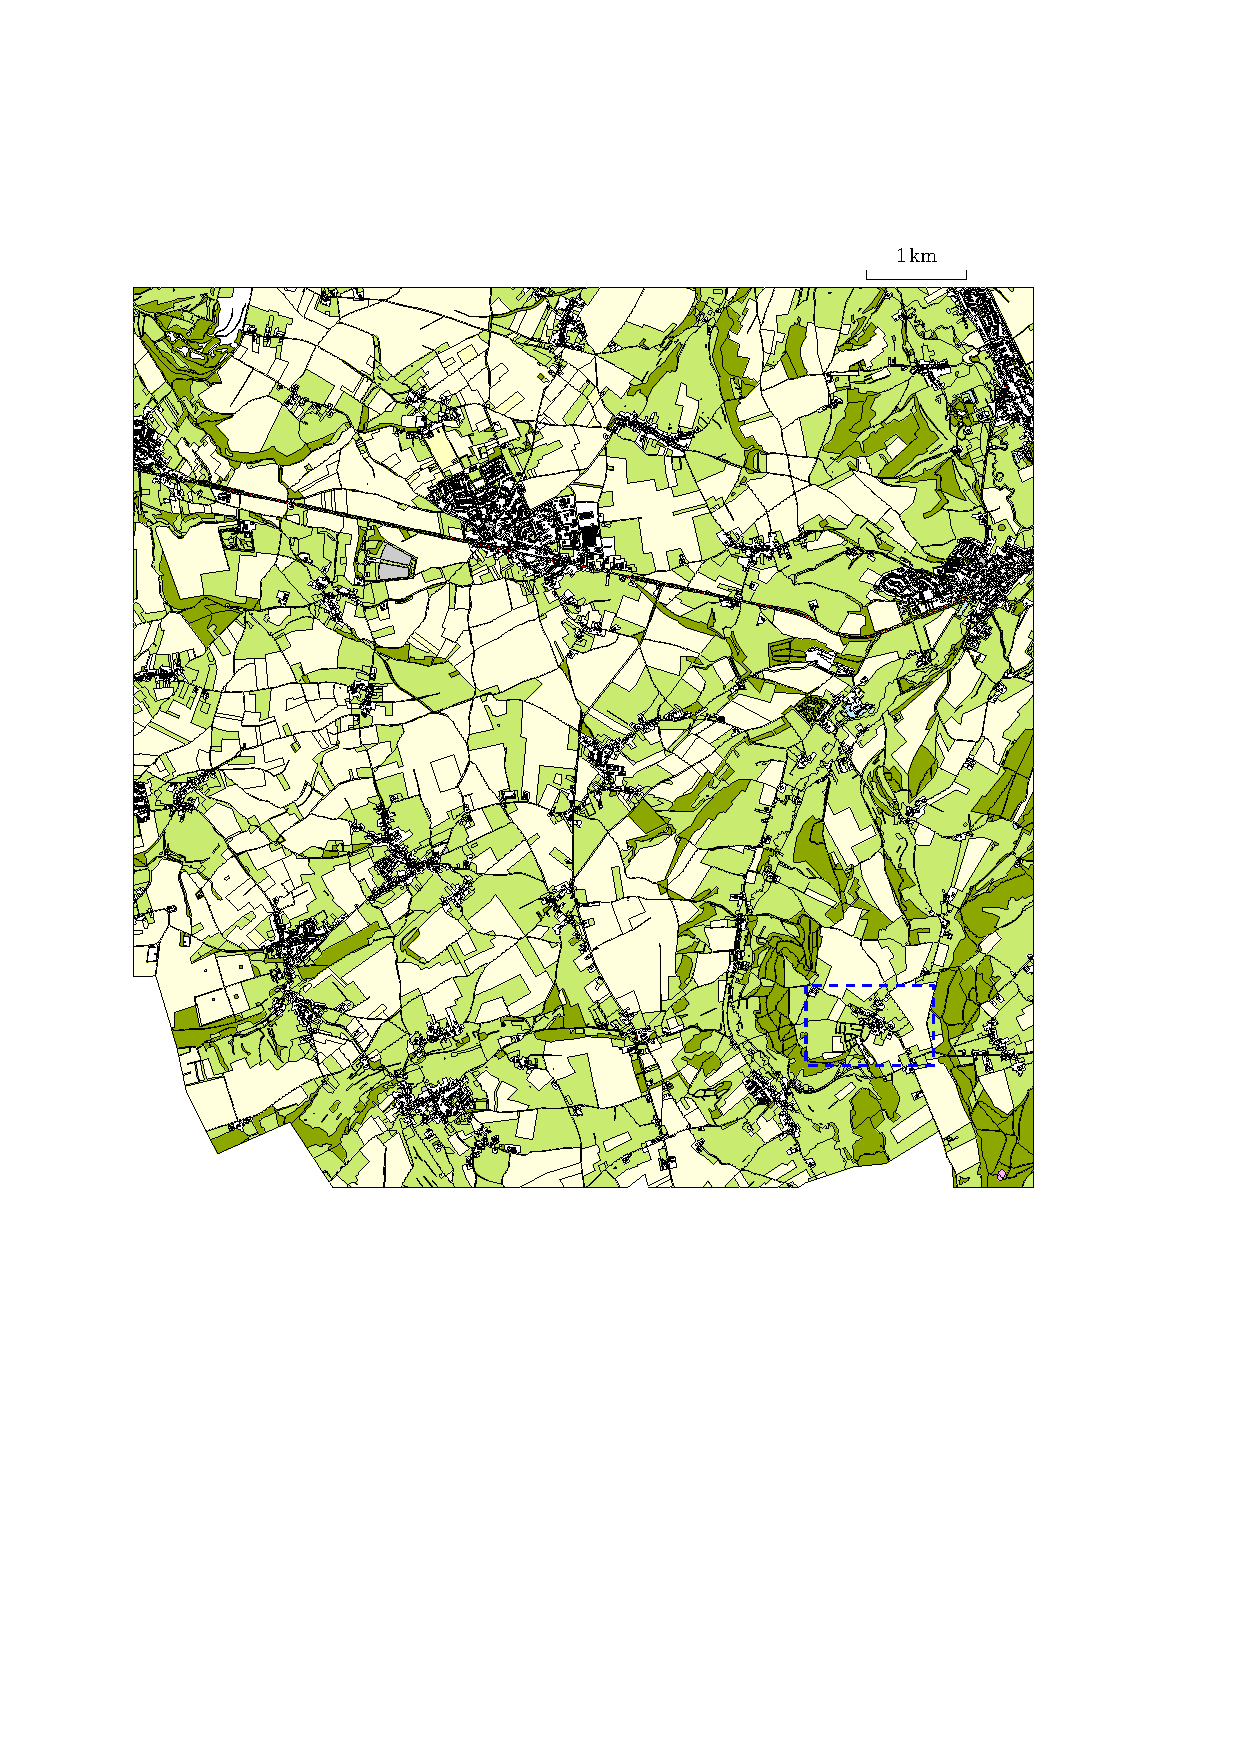
\includegraphics[page=1,draft=false,width=\linewidth,clip=true, trim = 12mm 14mm 2mm 0mm]{data}
\caption{
    The topographic map represents the place 
    in the south of Limburg, The Netherlands.
    There are $13{,}238$ parcels.
    The map is for scale $1:10{,}000$.}
\label{fig:data}
\end{figure}


\begin{figure}[tb]
\centering
%\begin{subfigure}[t]{\textwidth}
%\centering
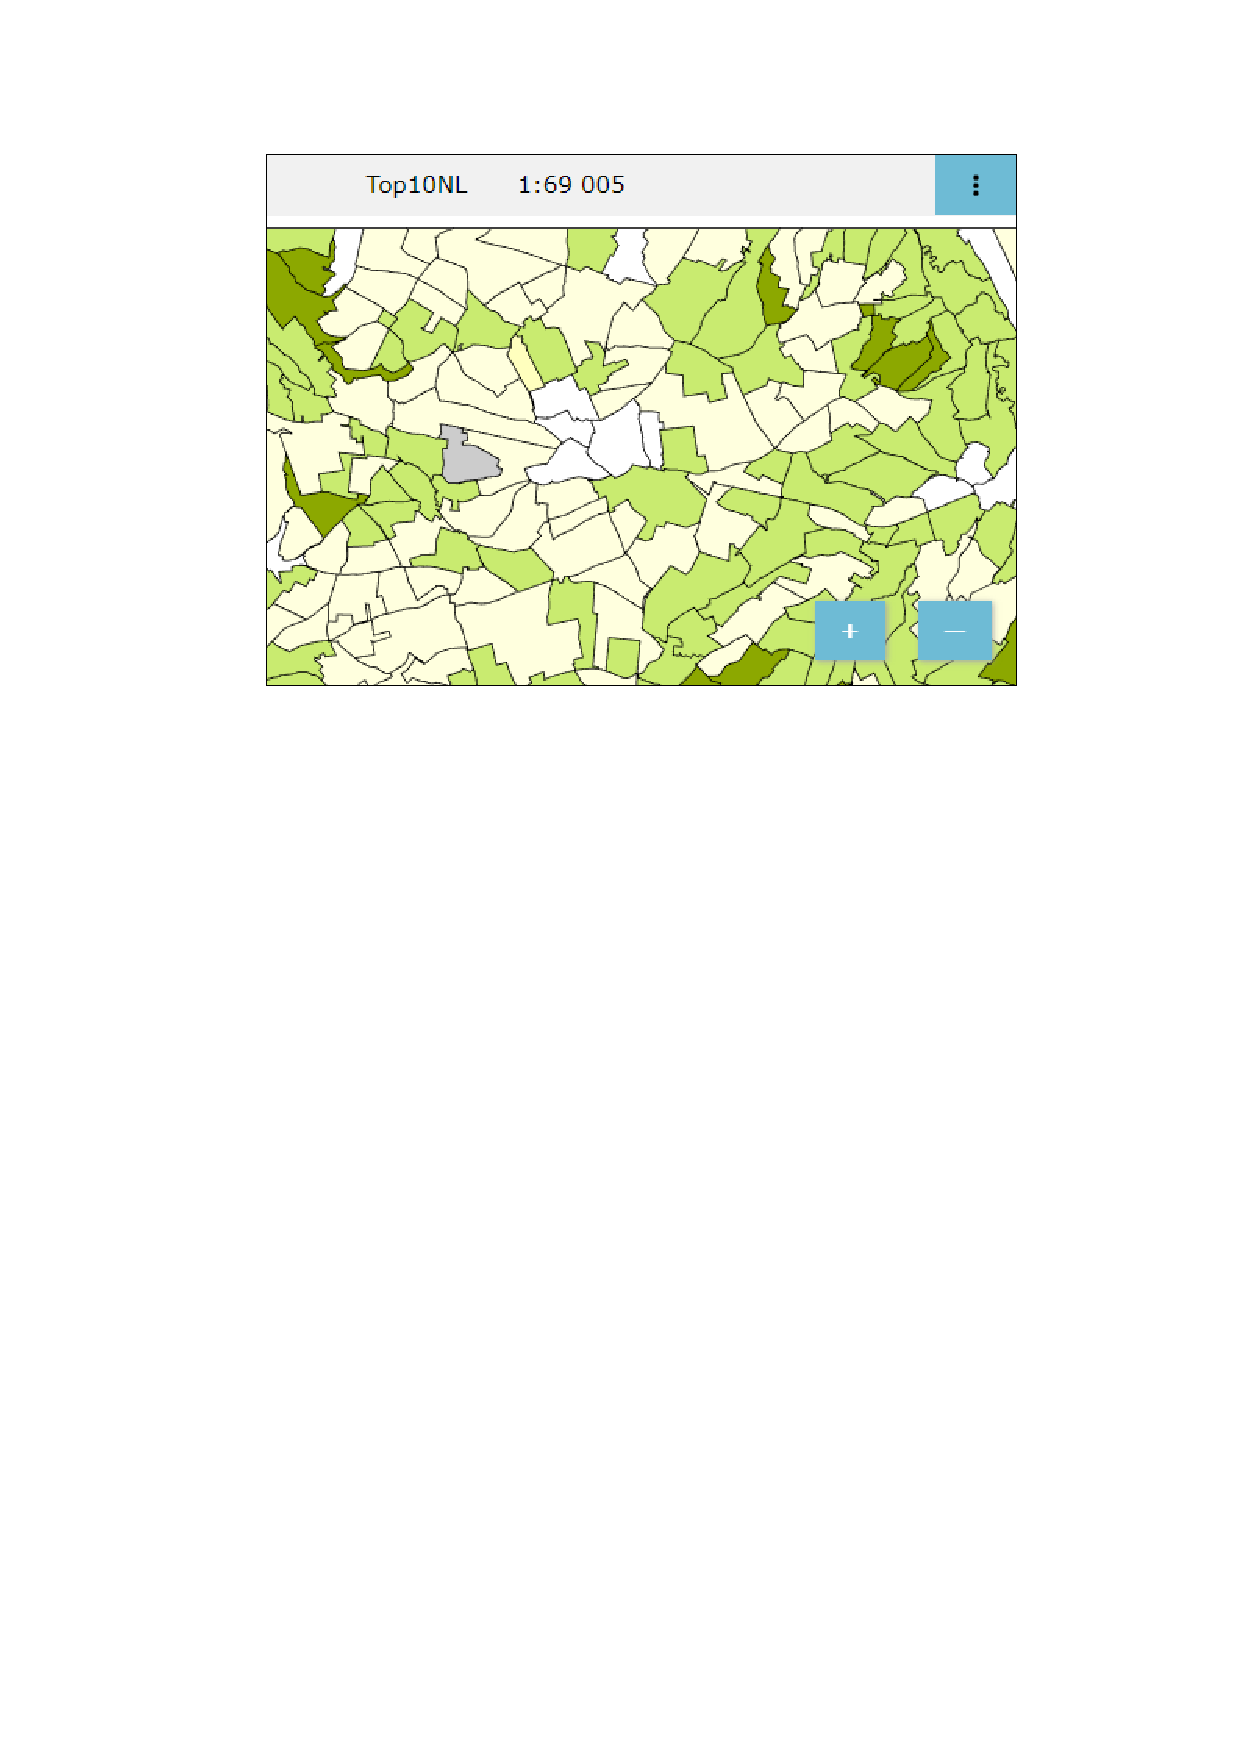
\includegraphics[page=1,scale=0.6]{case_study}
\caption{An overview map. The map is generated from the base map 
    by parallel merging with parameter~$r_\mathrm{parallel}= 0.01$.}
%\end{subfigure}
%\newline
%\vspace{0.5cm}
%\begin{subfigure}[t]{\textwidth}
%\centering
%\includegraphics[page=2,scale=0.6]{case_study}
%\caption{A part of the base map. The displayed place is marked 
%    by the dashed rectangle in \fig\ref{fig:data}.}
%%\end{subfigure}
%\caption{An example of our web map.}
\label{fig:web_map}
\end{figure}


\begin{figure}[tb]
\centering
\includegraphics[page=3,scale=0.6]{case_study}
\caption{
    A comparison of single merging (left) 
    and parallel merging (right, $r_\mathrm{parallel}= 0.1$).
    The slider can be moved to tune the widths of the two map canvases.
    Some sudden changes across the slider can be observed.
}
\label{fig:comparison}
\end{figure}



%In order to provide smooth merging
%so that map users can easily keep track of their area objects of interest,
%we merge by gradually expanding an area over another area
%(see \fig\ref{fig:intro}q).
%Note that the merging is independent of users' area objects of interest;
%the merging operations happen outside the region of interest
%are also realized by expanding.
%This expansion can be realized 
%by slicing the space-scale cube (SSC) of
%\fig\ref{fig:ssc}a.
%For example,  \fig\ref{fig:intro}q is obtained by slicing
%\fig\ref{fig:ssc}a at~$z= 250$.
%Smooth animations of zooming out are obtained by
%slicing an SSC from bottom to top.
%The details of slicing an SSC are illustrated in \citet{Meijers2020Web}.
%The SSCs of \fig\ref{fig:ssc} were built 
%based on the \emph{Eater} of \citet{Suba2014Merge}.
%The content of an SSC is stored in an OBJ file,
%and the OBJ file can be visualized by software ParaView
%(see \fig\ref{fig:ssc}).
%In \fig\ref{fig:ssc}, the $z$-coordinates are $100$ times of
%the state values in \fig\ref{fig:intro}.
%We did this multiplication so that the contents can be better observed;
%otherwise, the two SSCs will be very short when displayed in ParaView.
%
%
%Our strategy of presenting the static boundary (\ie~the exterior one) 
%is that we store the polylines and 
%draw them with width, 
%where the width is computed according to the map scale on the fly.
%We do not draw the common boundary of 
%a pair of areas that are being merged
%so that it is easy for map users 
%to identify the pairs of areas in transition. 
%
%
%
%\begin{figure*}[tb]
%\centering
%\includegraphics[page=1,scale=0.85]{introduction}
%\caption{A comparison of different scale-transition strategies.
%Each arrow inside the subfigures indicates a merging operation.
%The arrow in the right-hand side indicates the states of zooming out.
%%
%(a--c): All changes are processed in one go.
%(d--j): All changes are sequenced one by one rapidly.
%(k--o): Changes are grouped, resulting in more animation duration for every change.
%The numbers are the face IDs.
%}
%\label{fig:intro}
%\end{figure*}
%
%
%
%\begin{figure*}
%\centering
%\begin{subfigure}[t]{0.48\textwidth}
%\centering
%\includegraphics[page=4,width=0.95\linewidth]{methodology}
%\caption{The SSC of the single merging of \figs\ref{fig:intro}d--j.}
%\end{subfigure}
%\hfill
%\begin{subfigure}[t]{0.48\textwidth}
%\centering
%\includegraphics[page=5,width=0.95\linewidth]{methodology}
%\caption{The SSC of the parallel merging of \figs\ref{fig:intro}k--o}
%\end{subfigure}
%\caption{
%In the left SSC, only one merging event is happening 
%at a specific state ($z$-dimension), 
%while in the right SSC multiple merging events may happen at the same state.
%}
%\label{fig:ssc}
%\end{figure*}
%
%
%We define an \emph{event} as a single generalization operation, 
%such as merging an area into a neighbor.
%For example, \fig\ref{fig:intro}e is obtained from 
%\fig\ref{fig:intro}d by processing one merging event.
%Similarly, \fig\ref{fig:intro}l is obtained from 
%\fig\ref{fig:intro}k by processing two merging events.
%We define a \emph{step} as 
%a set of events happening at the same animation duration.
%For example, 
%\fig\ref{fig:intro}e is obtained from 
%\fig\ref{fig:intro}d by processing a step with one merging event.
%\fig\ref{fig:intro}l is obtained from 
%\fig\ref{fig:intro}k by processing a step with two merging events.
%In our method, a step is completely processed 
%before the next step takes place (all sequential).
%We define a \emph{state} as the point when a step starts or finishes.
%For example, there are seven states 
%in the merging sequence of \figs\ref{fig:intro}d--j
%(\ie~states 0, 1, 2, 3, 4, 5, and 6, from bottom to top)
%and five states in the merging sequence of \figs\ref{fig:intro}k--o 
%(\ie~states 0, 2, 4, 5, and 6).
%The value of a state is also the total number of events processed so far.
%
%
%We require that 
%the area objects involved in different merging events of the same step 
%must not be neighbors, 
%which makes the merging events independent from each other.
%There are two benefits of this independency.
%First, it is easy to maintain the topology of the map.
%When a pair of areas have been merged, 
%we must update the common boundaries with the surrounding adjacent areas.
%If an adjacent area is involved in another merging event,
%then it is complicated to update the adjacent area's boundaries
%for the two merging events.
%Second, users can keep track of their area objects of interest more easily
%than merging several areas into a single one.
%In order to realize the requirement,
%we block the neighbors of the areas once we have found an event.
%We show a greedy algorithm to find the parallel merging events for each step
%in \sect\ref{sec:greedy_algo}.
%Then, we integrate the events into the tGAP database tables
%(\sect\ref{sec:integrate_tgap}),
%followed by integrating the events into the SSC 
%(\sect\ref{sec:integrate_ssc}).
%In \sect\ref{sec:snap}, we show how to snap the zooming to valid states
%to avoid half-way merging animation 
%as stopping halfway will result in showing slivers in a static state.
%In \sect\ref{sec:zooming_duration}, we define 
%the animation duration of zooming from one state to another state.
%
%
%
%\subsection{A greedy algorithm}
%\label{sec:greedy_algo}
%
%In the greedy algorithm, 
%we need to obtain the most compatible neighbor for a given area.
%There are many ways of defining the most compatible neighbor.
%For example, \citet{Cheng2006} proposed three choices, i.e.,
%the neighbor has the largest size, 
%shares the longest boundary with the least important area,
%or has the closest class to the least important area. 
%\citet{Peng2017AStar} proposed that 
%the most compatible neighbor should have a close class
%to the least important area
%and the combination of the two areas should be compact;
%they defined the class distance based on a binary tree
%according to the codes of the classes.
%We define the importance and the compatibility as
%the same as \citet{vanOosterom2005,vanPutten1998NewGAP}.
%That is, the importance of an area is the multiplication 
%of its size and its class weight.
%The compatibility value between a pair of areas is 
%the multiplication of the common boundary's length and 
%the class similarity of the two areas.
%\appx\ref{appx:create_tables} shows our implementation of
%computing the weight values and the class similarities.
%
%
%
%\fig\ref{fig:greedy_framework} shows the flowchart of our greedy algorithm.
%The process starts with state~$s=0$ and a detailed map of area objects, $|M_0|$.
%Parallel parameter~$r_\mathrm{parallel}$ specifies 
%the proportion (\ie~percentage, when multiplied by~$100$) of area objects that
%we expect to merge parallelly.
%As a value of percentage, 
%$r_\mathrm{parallel}$ is in the range from~$0\%$ to~$100\%$,
%which means~$r_\mathrm{parallel} \in [0,1]$.
%Expression~$|M_s|$ denotes the number of area objects of the map at state~$s$.
%If there is more than one area ($|M_s|>1$),
%then we start finding merging events.
%We first compute the number of areas that we expect to merge by
%\begin{equation}
%\label{eq:n_target}
%n_\mathrm{target} =
%\lceil r_\mathrm{parallel} \cdot |M_s| \rceil,
%\end{equation}
%where the ceiling function guarantees~$n_\mathrm{target}\ge 1$.
%That is to say, we find at least one event for each step.
%When~$n_\mathrm{target} > 1$, however,
%we cannot always find~$n_\mathrm{target}$ events
%because some areas may be blocked as explained before
%(also see \fig\ref{fig:blocked_polygons}).
%Therefore, we use variable~$n_\mathrm{event}$
%to represent the number of events that actually happened within the step. 
%
%
%\begin{figure*}[tb]
%\centering
%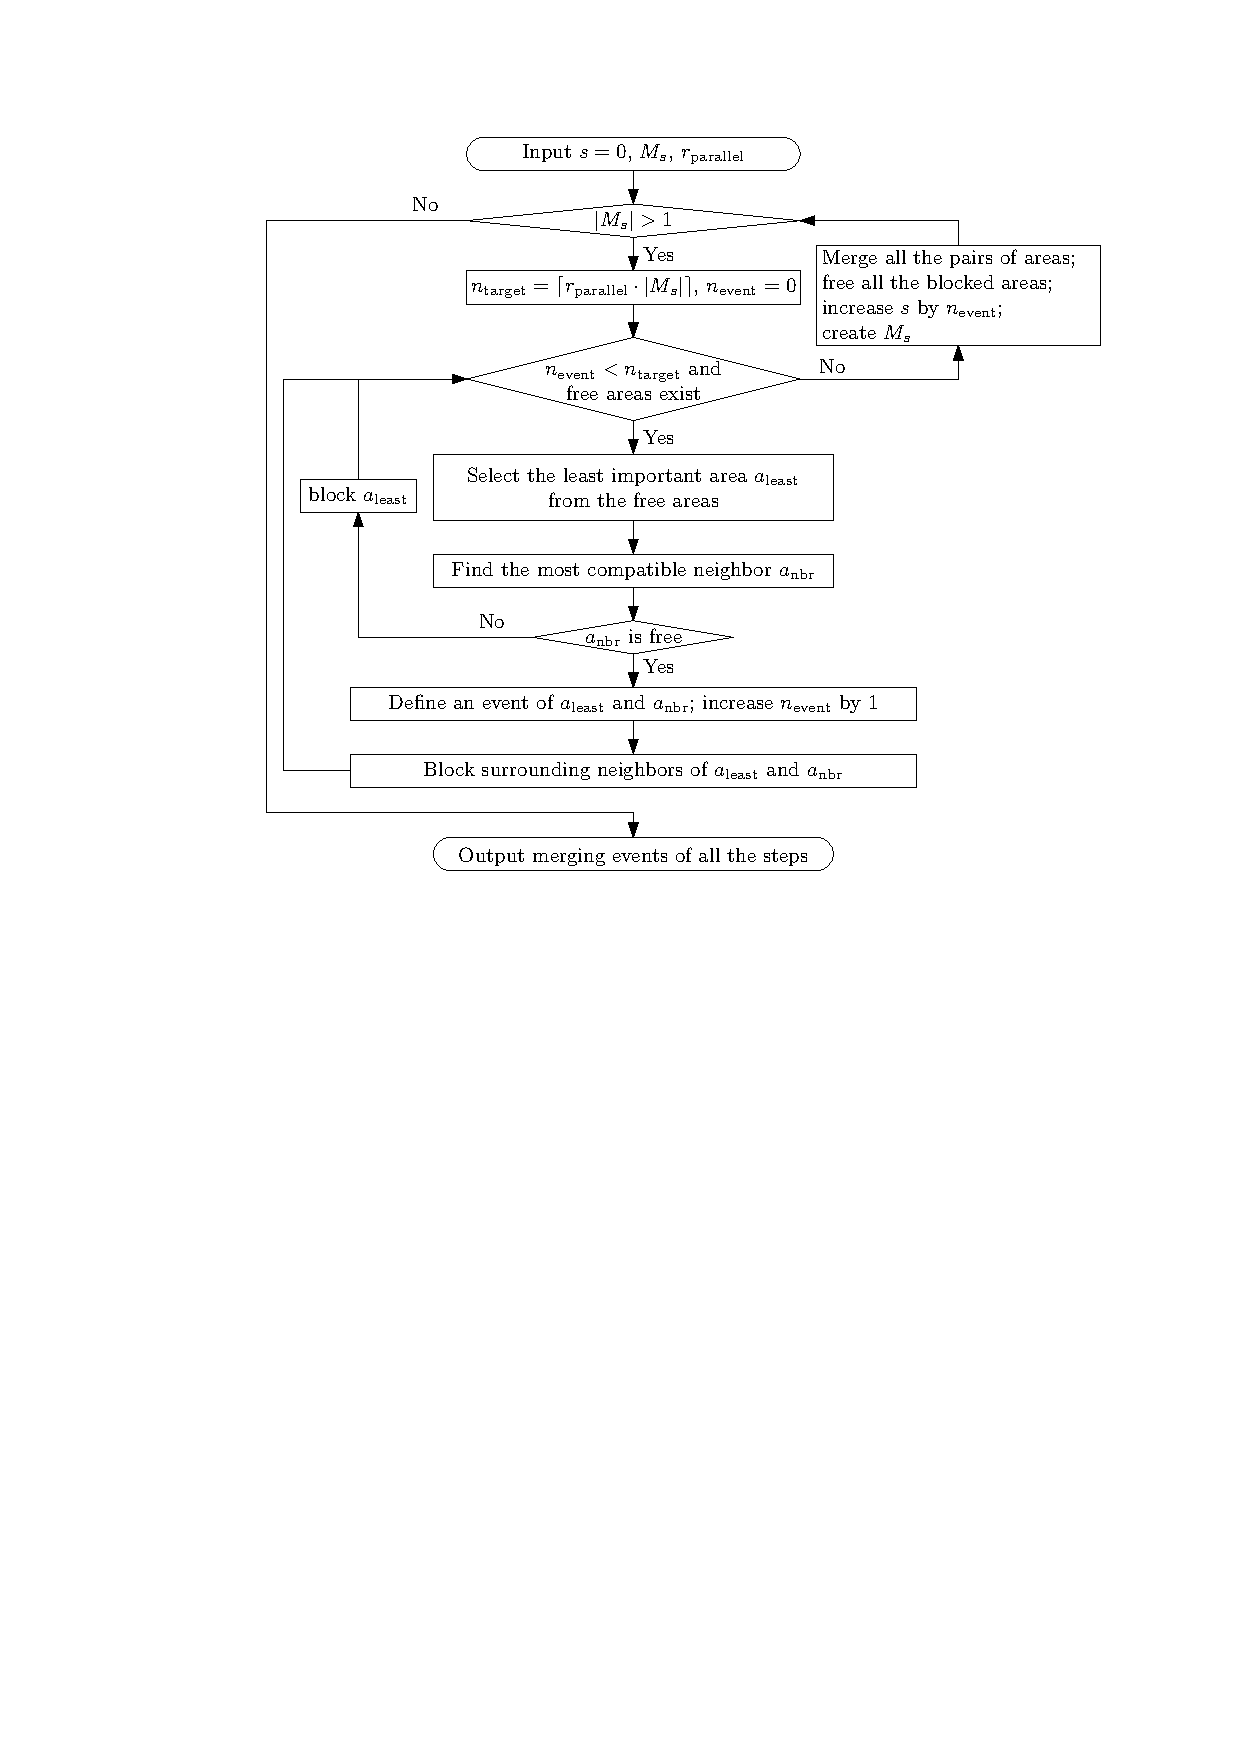
\includegraphics[page=1]{methodology}
%\caption{The flowchart of our greedy algorithm.
%}
%\label{fig:greedy_framework}
%\end{figure*}
%
%
%\begin{figure*}[tb]
%\centering
%\includegraphics[page=2]{methodology}
%\caption{The process of finding parallel merging events for a step.
%    (a) From all the free areas,
%	the least important one is selected to merge into
%	its most compatible neighbor.
%	Then the surrounding areas are blocked (marked by the crosses).
%	(b) Next, the least important area from the remaining free areas
%	is selected to merge with the most compatible neighbor,
%	and the surrounding areas are also blocked.
%}
%\label{fig:blocked_polygons}
%\end{figure*}
%
%If we have not found $n_\mathrm{target}$ events 
%($n_\mathrm{event} < n_\mathrm{target}$)
%and there are still free areas,
%then we go on looking for merging events.
%We select the least important area~$a_\mathrm{least}$
%from the free areas.
%An area is \emph{free} if 
%it is not involved in an event and is not blocked.
%We also find~$a_\mathrm{least}$'s 
%most compatible neighbor~$a_\mathrm{nbr}$.
%If area~$a_\mathrm{nbr}$ is also free, 
%we define an event of areas~$a_\mathrm{least}$ and~$a_\mathrm{nbr}$.
%Then, we increase the number of events, $n_\mathrm{event}$, by 1.
%We block the surrounding neighbors of~$a_\mathrm{least}$ and~$a_\mathrm{nbr}$
%(see \fig\ref{fig:blocked_polygons}a).
%Note that the area shares only a vertex 
%with the least important area is not blocked.
%If area~$a_\mathrm{nbr}$ is not free,
%then it must be blocked because of the previously found events.
%In this case, we block $a_\mathrm{least}$ for now
%so that areas~$a_\mathrm{least}$ and~$a_\mathrm{nbr}$ 
%may merge in the next step.
%Then, we continue to find more merging events and to block more areas
%(see \fig\ref{fig:blocked_polygons}b).
%
%If we have found~$n_\mathrm{target}$ events 
%or there is no free area anymore,
%then finding merging events of the step finishes.
%We parallelly merge all the pairs of areas of the found events
%to generate new areas,
%free all the blocked areas,
%increase state~$s$ by value~$n_\mathrm{event}$,
%and create map~$M_s$ based on the new areas and the freed areas.
%Then, finding merging events for the next step starts.
%This iteration of finding completes 
%until there is only one area left on the map ($|M_s|=1$).
%The merging events will be stored as records in tGAP database tables
%(see \fig\ref{fig:uml_tgap}).
%\figs\ref{fig:intro}k--o show a sequence of four merging steps
%obtained by our greedy algorithm,
%where parallel parameter~$r_\mathrm{parallel}$ is set to~$0.3$
%(Note that this is an extremely high value, 
%just used to explain the principle in an artificial simple example).
%
%
%
%\begin{figure*}[tb]
%\centering
%\includegraphics[page=3]{methodology}
%\caption{The UML diagram of the classes stored in tGAP database tables.
%This diagram is a slightly improved version of \citet[\p159]{Meijers2011Thesis}.
%In the face table, property \emph{pip\_geometry} 
%stores a point (usually the center) in the face (polygon).
%The geometry of a face can be obtained by calling function \emph{getGeometry()}.
%We do not store the face geometry because we want to avoid redundancy,
%as the edges already stores the sequences of points.
%}
%\label{fig:uml_tgap}
%\end{figure*}
%
%
%\subsection{Integrating the parallel events into the tGAP database tables}
%\label{sec:integrate_tgap}
%
%\citet[\p159]{Meijers2011Thesis} designed three tables 
%to record the information of
%faces, edges, and face hierarchies, 
%which together form a tGAP.
%For example, the face table contains columns \emph{face\_id}, 
%\emph{imp\_low}, \emph{imp\_high}, \emph{imp\_own},
%\emph{feature\_class}, \emph{area}, and \emph{mbr\_geometry}.
%We add columns \emph{state\_low} ($s_\mathrm{low}$) 
%and \emph{state\_high} ($s_\mathrm{high}$) into the table 
%so that it is easy to see when a face should appear or disappear 
%(see \tbls\ref{tbl:face_tgap}a and~\ref{tbl:face_tgap}b,
%where all other columns, except face\_id, are hidden).
%For zooming out, a face should appear, 
%from the merging of two faces,
%when the slicing arrives at the low state.
%When the slicing arrives at the high state,
%the face should have been merged with another area.
%Comparing between the tables of single merging 
%(\figs\ref{fig:intro}d--j)
%and parallel merging (\figs\ref{fig:intro}k--o),
%we observed some differences of the values.
%For example, the $s_\mathrm{high}$ values of faces~1 and~2 are changed from~1 to~2
%(see \tbl\ref{tbl:face_tgap}).
%Also, the $s_\mathrm{low}$ value of face~8 is changed from~1 to~2
%(see \tbl\ref{tbl:face_tgap}).
%Similarly to the face tables, 
%the columns and records of both the edge table and the face-hierarchy table 
%will be changed accordingly.
%
%
%\begin{table*}[tb]
%\caption{Some columns of the face tables. 
%    Columns~$s_\mathrm{low}$, $s_\mathrm{merge}$, 
%    and~$s_\mathrm{high}$ show the states 
%    when the faces appear, when the faces start to disappear, and
%    when the faces completely disappear.    
%    In table~(b), the different values from table~(a) are underlined.
%    Column~$s_\mathrm{merge}$ is not really stored in the database.
%    We show the column so that it is easy to see the differences 
%    between the $s_\mathrm{low}$ values and the $s_\mathrm{merge}$ values.
%    }
%\label{tbl:face_tgap}
%\begin{subtable}{0.48\textwidth}
%\caption{The face table of the single merging 
%    shown in \figs\ref{fig:intro}d--j.}
%\centering
%\begin{tabular}{cccc}
%\toprule
%$f_\mathrm{id}$& $s_\mathrm{low}$    & $s_\mathrm{merge}$ & $s_\mathrm{high}$ \\ \midrule
%1       &     0         &     0         &     1       \\
%2       &     0         &     0         &     1       \\
%3       &     0         &     1         &     2       \\ 
%4       &     0         &     4         &     5       \\
%5       &     0         &     3         &     4       \\
%6       &     0         &     2         &     3       \\         
%7       &     0         &     2         &     3       \\
%8       &     1         &     1         &     2       \\
%9       &     2         &     5         &     6       \\         
%10      &     3         &     3         &     4       \\
%11      &     4         &     4         &     5       \\ 
%12      &     5         &     5         &     6       \\ 
%13      &     6         &    ---        &    ---      \\
%\bottomrule
%\end{tabular}
%\end{subtable}
%%
%\hfill
%%
%\begin{subtable}{0.48\textwidth}
%\caption{The face table of the parallel merging 
%    shown in \figs\ref{fig:intro}k--o.}
%\centering
%\begin{tabular}{cccc} %\underbar{2}
%\toprule
%$f_\mathrm{id}$ & $s_\mathrm{low}$   & $s_\mathrm{merge}$ & $s_\mathrm{high}$ \\ \midrule
%1       &     0         &     0         &\underbar{2} \\
%2       &     0         &     0         &\underbar{2} \\
%3       &     0         & \underbar{2}  &\underbar{4} \\ 
%4       &     0         &     4         &     5       \\
%5       &     0         & \underbar{2}  &     4       \\
%6       &     0         & \underbar{0}  &\underbar{2} \\         
%7       &     0         & \underbar{0}  &\underbar{2} \\
%8       & \underbar{2}  & \underbar{2}  &\underbar{4} \\
%9       &     2         &     5         &\underbar{6} \\         
%10      & \underbar{4}  & \underbar{2}  &\underbar{4} \\
%11      &     4         &     4         &     5       \\ 
%12      &     5         &     5         &     6       \\ 
%13      &     6         &    ---        &    ---      \\
%\bottomrule
%\end{tabular}
%\end{subtable}
%\end{table*}
%
%
%\subsection{Integrating the parallel events into the SSC}
%\label{sec:integrate_ssc}
%
%Recall that we merge a pair of areas by expanding over 
%the less important area from the neighbor.
%The Eater of \citet{Suba2014Merge} is used to 
%triangulate the less important area and to tilt the triangles.
%Then the tilted triangles are integrated into the SSC
%(see \fig\ref{fig:ssc})
%so that we can slice the SSC to achieve smooth merging.
%For the case of single merging,
%if a pair of areas have state-high value~$s_\mathrm{high}$,
%then the merging animation 
%always starts at state~$s_\mathrm{merge}=s_\mathrm{high}-1$
%(see \tbl\ref{tbl:face_tgap}a).
%The less important area completely disappears
%at state~$s_\mathrm{high}$.
%In the face table, a row will be added to record the new area, 
%and its $s_\mathrm{low}$ value will be the previous~$s_\mathrm{high}$ value.
%The new area takes the combined place of the pair of areas.
%Take \ref{fig:intro} as an example, 
%area~1 is merged into area~2 (\figs\ref{fig:intro}d), 
%and area~8 is generated to take the combined place (\figs\ref{fig:intro}e).
%The tilted triangle is the one spans 
%from~$z= 0$ to~$z=100$ (\ie~from state~0 to state~1)
%in \fig\ref{fig:ssc}a.
%In \tbl\ref{tbl:face_tgap}a, 
%the~$s_\mathrm{low}$ value of area~8 is 1,
%which is the~$s_\mathrm{high}$ values of areas~1 and~2.
%%Note that the state\_low values of the two areas do not matter 
%%because those values respectively indicate the states that
%%the two areas appear;
%%those values can be much smaller 
%%than value~$s_\mathrm{high}-1$.
%
%For the case of parallel merging,
%if a step consists of~$n_\mathrm{event}$ events and 
%the step finishes at state~$s_\mathrm{high}$, then the step starts 
%at state~$s_\mathrm{merge}=s_\mathrm{high} - n_\mathrm{event}$.
%The reason is that if the~$n_\mathrm{event}$ events 
%would happen sequentially (\ie~single merging),
%then they would take place 
%from state~$s_\mathrm{high} - n_\mathrm{event}$ to state~$s_\mathrm{high}$.
%When all the events take place parallelly in the same step, 
%each of the events can share its merging duration.
%%there is a less important area in each of the parallel events of a merging step.
%%If the number of parallel events is~$n_\mathrm{event}$,
%%then there are~$2n_\mathrm{event}$ areas 
%%with the same state\_high value, say,~$s_\mathrm{high}$
%%because each merging event involves two areas.
%%The merging animations of all the parallel events
%%start at state~$s_\mathrm{merge}=s_\mathrm{high} - n_\mathrm{event}$
%%and finishes at state~$s_\mathrm{high}$.
%%By definition, the parallel events of a merging step 
%%happen during the same animation time.
%%In other words, the areas involved in those parallel events have 
%%the same state\_merge value ($s_\mathrm{merge}$) and 
%%the same state\_high value ($s_\mathrm{high}$).
%%The reverse is also true.
%%If some areas have the same state\_high value,
%%then those areas happen during the same animation time 
%%(involved in the parallel events of the same step).
%%The reason is that, according to our requirement,
%%a step can start only when the previous step stops.
%%Thus, the merging events finishing at the same state cannot from different steps.
%%of these areas 
%%will finish at state~$s_\mathrm{high}$,
%%and no merging event will start earlier or later than state~$s_\mathrm{merge}$
%%because we required that the next step starts only when a step stops.
%%Given the fact that the merging duration for zooming 
%%between states~$s_\mathrm{merge}$ and~$s_\mathrm{high}$ is fixed,
%As a result,
%each of the parallel events has more time to take place
%than the events would happen sequentially.
%In other words, for a merging step,
%each of the events has more time to take place 
%if there are more parallel events.
%
%In order to build the SSC for parallel merging,
%we need the~$s_\mathrm{merge}$ value for each of the merging steps
%so that we know from which state 
%the triangles of the less important areas should be tilted.
%A simple way is to add a column, say, $s_\mathrm{merge}$
%into the face table during generating the tGAP, 
%as done in \tbl\ref{tbl:face_tgap}.
%Then, the states of starting merging can be recorded into the column.
%However, we would like to avoid unnecessary columns to save storage.
%Therefore, we compute~$s_\mathrm{merge}$ values 
%based on the~$s_\mathrm{high}$ values
%on the fly when building the SSC.
%As an event involves two areas,
%the number of events finishing at state~$s_\mathrm{high}$ can be calculated by
%\begin{equation*}
%\label{eq:n_event_state}
%n_\mathrm{event} (s_\mathrm{high}) = 
%\frac{\sum\limits_{s \in S_\mathrm{high}} [s=s_\mathrm{high}]}{2},
%\end{equation*}
%where notation~$S_\mathrm{high}$ denotes the set of values
%recorded in column~$s_\mathrm{high}$ of the face table
%(\eg~\tbl\ref{tbl:face_tgap}b).
%Expression~$[s=s_\mathrm{high}]$ returns~$1$ if the two values are equal 
%and returns~$0$ otherwise.
%As illustrated before, the state at which the parallel merging starts 
%can be computed by
%\begin{equation*}
%\label{eq:s_merge_state}
%s_\mathrm{merge} (s_\mathrm{high}) = s_\mathrm{high} - n_\mathrm{event} (s_\mathrm{high}).
%\end{equation*}
%
%
%
%Take the case of \tbl\ref{tbl:face_tgap}b for example,
%we have~$S_\mathrm{high} = \{2, 2, 4, 5, 4, 2, 2, 4, 6, 4, 5, 6\}$, 
%$n_\mathrm{event} (4) = 2$, and~$s_\mathrm{merge} (4) = 2$.
%Therefore, there are two merging events finishing at state~$4$,
%\ie~event of merging area 3 into area~8 and 
%event of merging area~5 into area~10 
%(also see \figs\ref{fig:intro}l and~\ref{fig:intro}m).
%The merging animation takes place from state~$2$ to state~$4$.
%This merging can be also observed from 
%the two tilted triangles spanning from~$z = 200$ to~$z = 400$ 
%in \fig\ref{fig:ssc}b.
%In merging sequence of \figs\ref{fig:intro}d--j, 
%the animation of merging area~3 into area~8 
%takes place from state~$1$ to state~$2$
%(also see the tilted triangle spanning from~$z = 100$ to~$z = 200$ 
%in \fig\ref{fig:ssc}a), and 
%the animation of merging area~5 into area~10
%takes place from state~$3$ to state~$4$
%(also see the tilted triangle spanning from~$z = 300$ to~$z = 400$ 
%in \fig\ref{fig:ssc}a).
%As a result, the animation duration of merging area~3 into area~8 of 
%sequence \figs\ref{fig:intro}k--o
%is almost twice as that of sequence \figs\ref{fig:intro}d--j.
%We say \emph{almost} because the animation duration is also dependent on 
%the current state of the map
%(see \sect\ref{sec:zooming_duration}).
%
%
%\subsection{Snapping to a valid state}
%\label{sec:snap}
%
%For a zooming action based on the SSC, 
%we always snap the map to a valid state.
%In this way, users will not see a merging operation stops half-way
%and will not see transition artifact (such as slivers).
%Take the sequence of \fig\ref{fig:intro}k--o for example, 
%the merging animation should stop at 
%either \ref{fig:intro}k or \ref{fig:intro}l,
%but not at \ref{fig:intro}r.
%Note that some states are not valid because of the parallel events.
%For example, state~$1$ is not valid 
%for the sequence of \fig\ref{fig:intro}k--o.
%In that example, the list of valid states 
%is~$S_\mathrm{valid} = [0, 2, 4, 5, 6]$.
%In order to snap to one of the valid states after a zooming operation,
%we have to communicate them to the client side. 
%There are multiple options. 
%The most simple one assumes that, 
%during the creation of the parallel SSC, 
%we can always perform the~$n_\mathrm{target}$ number of events in all steps. 
%In that case, we just have to communicate 
%the number of areas and the ratio~$r_\mathrm{parallel}$. 
%In case of high value ratios (\eg~$r_\mathrm{parallel} > 0.01$), 
%this assumption may be incorrect. 
%We then have to communicate the valid states by sending them explicitly. 
%Because this list may get rather large,
%we only send exceptions.
%\appx\ref{appx:communicate_valid_states} shows the details of the technique.
%As a result, the list of valid states~$S_\mathrm{valid}$ is sent to the client side.
%
%
%According to how much a user has zoomed,
%the target scale, say, $1:S_\mathrm{t}$ can be computed.
%%According to \citet{Huang2016Webmap},
%%the number of merging events that should be processed can be computed by
%\citet{Huang2016Webmap} suggested that 
%the average density of the original map should be preserved 
%for a smaller-scale map.
%Their suggestion is based on the assumption that 
%the area density of the base map is well designed, which is reasonable.
%We use variable~$A_\mathrm{real}$ to denote the total areal size of 
%all the area objects in reality.
%Then, the size on screen at scale~$1:S_\mathrm{t}$ 
%is~$A_\mathrm{real} \big/ S^2_\mathrm{t}$.
%In order to keep the density, we require
%\begin{equation}
%\label{eq:equal_density}
%\frac{N_\mathrm{b}}{A_\mathrm{real} \big/ S^2_\mathrm{b}} =
%\frac{N_\mathrm{b}-E_\mathrm{t}}{A_\mathrm{real} \big/ S^2_\mathrm{t}},
%\end{equation}
%where parameter~$N_\mathrm{b} = |M_0|$ 
%is the number of areas on the base map,
%parameter~$S_\mathrm{b}$ is the scale denominator of the base map,
%and variable~$E_\mathrm{t}$ is the total number of events 
%happening from the base map to the map at scale~$1:S_\mathrm{t}$.
%\eq\ref{eq:equal_density} yields
%\begin{equation}
%\label{eq:E_t}
%E_\mathrm{t} = N_\mathrm{b} \left(1-\frac{S^2_\mathrm{b}}{S^2_\mathrm{t}}\right),
%\end{equation}
%In our example regarding to list of valid states~$\mathrm{S_\mathrm{valid}}$,
%if event number~$E_\mathrm{t} \le 0$, the base map should be presented;
%if $E_\mathrm{t} \ge 6$ (\ie~the last value of list~$L_\mathrm{event}$),
%the map with the final single area should be presented.
%Otherwise, if $0<E_\mathrm{t} < 6$, we snap event number~$E_\mathrm{t}$ 
%to the closest value (measured in events) of list~$S_\mathrm{valid}$,
%which is denoted by~$E_\mathrm{t,snap}$.
%The scale denominator corresponding to event number~$E_\mathrm{t,snap}$
%can be computed by 
%\begin{equation}
%\label{eq:S_t_snap}
%S_\mathrm{t,snap} = S_\mathrm{b} \sqrt{\frac{N_\mathrm{b}}{N_\mathrm{b}-E_\mathrm{t,snap}}}.
%\end{equation}
%where this equation is an inverse function of \eq\ref{eq:E_t}.
%At the end of the zooming action, 
%the map will snap to state~$s_\mathrm{t,snap}$
%at scale~$1:S_\mathrm{t,snap}$.
%Note that state~$s_\mathrm{t,snap}$ always has 
%the same value as event number~$E_\mathrm{t,snap}$.
%
%
%
%%\subsection{Line simplification (smoothly moving vertices for the SSC)}
%
%
%\subsection{Animation duration of a step}
%\label{sec:zooming_duration}
%
%When users are zooming from a scale to another scale,
%some steps take place to change the map from a state to another one.
%We define the \emph{zooming duration} as the amount of 
%animation time that the map reacts to one ``click'' of the mouse wheel.
%The zooming duration often is the sum of 
%the \emph{animation durations} of several merging steps.
%The animation duration of each event depends on 
%the number of events between the two states,
%the \emph{zooming factor} of the scale, and 
%the \emph{zooming duration}.
%On the one hand, the animation duration should not be too short 
%as then the animation will be too fast. 
%On the other hand, if the animation takes too long, 
%the map will not be interactive, and users will be ``frustrated''.
%\citet[][\sect4.3]{Meijers2020Web} 
%have introduced the zooming factor and the zooming duration.
%They allowed users to set the two parameters,
%which is also the case in this paper
%(see \fig\ref{fig:interaction_settings}).
%As no paper has recommended values for 
%the zooming factor or the zooming duration,
%we respectively set the default values to $1$ and $1\,$s, 
%which performed well according to our experience.
%This section formalizes the relationship of the animation duration,
%the zooming duration, the zooming factor, and the number of events.
%In a zooming duration, there can be many merging steps,
%no matter single merging or parallel merging.
%The following calculation is based on the setting that
%a zooming duration is divided equally by its merging steps
%(\citet[][\sect6.7]{Suba2017Thesis} showed some other possible settings).
%In other words,
%the steps happen sequentially and take the same amount of animation duration.
%Note that the steps from different zooming durations 
%may have different animation durations.
%%In the following calculation, 
%%we assume that we can always find the target number 
%%(see \eq\ref{eq:n_target})
%%of events for all the steps.
%%If there are exceptions, 
%%then the following calculation should be adjusted accordingly.
%
%\begin{figure}[tb]
%\centering
%\includegraphics[page=6,scale=0.6]{methodology}
%\caption{Our panel of settings. 
%Among others, one can set how much to zoom when scrolling the mouse wheel 
%and set the zooming duration.}
%\label{fig:interaction_settings}
%\end{figure}
%
%
%Let~$f_\mathrm{zoom}$ be the zooming factor, and 
%let~$t_\mathrm{zoom}$ be the zooming duration.
%Let~$1:S_\mathrm{t,snap}$ be the snapped scale before the zooming operation, and 
%let~$1:S_\mathrm{o}$ be the zoomed out scale (not snapped yet).
%For zooming out, we define the relationship 
%between the two scale denominators as
%\begin{equation}
%\label{eq:S_o}
%S_\mathrm{o} = S_\mathrm{t,snap} (1 + f_\mathrm{zoom}).
%\end{equation}
%For scale~$1:S_\mathrm{o}$, we compute the number of events
%that should be processed from the base map by
%\begin{equation*}
%\label{eq:E_o}
%E_\mathrm{o} = N_\mathrm{b} \left(1-\frac{S^2_\mathrm{b}}{S^2_\mathrm{o}}\right),
%\end{equation*}
%which is according to \eq\ref{eq:E_t}.
%As the value of~$E_\mathrm{o}$ may be not an integer, 
%we snap it to a valid state
%(see \sect\ref{sec:snap}),
%and we have a snapped value~$E_\mathrm{o,snap}$.
%Then, we compute scale denominator~$S_\mathrm{o,snap}$
%by \eq\ref{eq:S_t_snap}.
%According to \eq\ref{eq:E_t}, we have merged~$E_\mathrm{t,snap}$ areas 
%when arriving at scale~$1:S_\mathrm{t,snap}$.
%The event number of zooming out
%from scale~$1:S_\mathrm{t,snap}$ to scale~$1:S_\mathrm{o,snap}$ is
%%$
%\begin{equation*}
%\label{eq:N_event}
%N_\mathrm{event} = 
%E_\mathrm{o,snap} - E_\mathrm{t,snap}.
%\end{equation*}
%%$
%%Accordingly, we can compute scale denominator~$S_\mathrm{o,snap}$
%%by \eq\ref{eq:S_t_snap}
%Recall that zooming duration~$t_\mathrm{zoom}$ is for zooming from 
%from scale~$1:S_\mathrm{t,snap}$ to scale~$1:S_\mathrm{o}$.
%As the map is actually zooming to~$1:S_\mathrm{o,snap}$,
%we adjust the zooming duration to
%\begin{equation*}
%\label{eq:E_i}
%t_\mathrm{snap}= t_\mathrm{zoom} 
%%\frac{n_\mathrm{event}}
%\frac{N_\mathrm{event}}
%{E_\mathrm{o} - E_\mathrm{t,snap}}.
%\end{equation*}
%%\begin{equation}
%%\label{eq:n_event}
%%n_\mathrm{event} 
%%= E_\mathrm{o} - E_\mathrm{t,snap}
%%= N_\mathrm{b} S^2_\mathrm{b} \left(\frac{1}{S^2_\mathrm{t,snap}} - \frac{1}{S^2_\mathrm{o}}\right).
%%\end{equation}
%That is to say, the~$E_\mathrm{o,snap} - E_\mathrm{t,snap}$ events will happen 
%in time duration~$t_\mathrm{snap}$.
%If the events happen sequentially (each step consists of a single event), 
%then the animation duration of each event is
%\begin{equation}
%\label{eq:t_single}
%t_\mathrm{single}   = \frac{t_\mathrm{snap}}{N_\mathrm{event}} 
%                    = \frac{t_\mathrm{zoom}}{E_\mathrm{o} - E_\mathrm{t,snap}}.
%\end{equation}
%
%If we parallel these events, 
%then we will have fewer steps and 
%each event has more time to take place.
%Let~$n_\mathrm{step}$ be the number of steps in a zooming duration.
%If we are lucky enough so that
%expression~$r_\mathrm{parallel} \cdot |M_s|$ of \eq\ref{eq:n_target}
%always returns an integer, 
%then we do not need the ceiling function of \eq\ref{eq:n_target}
%(if we are not that lucky, the value of~$n_\mathrm{step}$ will be slightly different).
%We have 
%\begin{equation*}
%%\label{eq:n_event}
%N_\mathrm{t,snap} (1-r_\mathrm{parallel})^{n_\mathrm{step}} = N_\mathrm{o,snap},
%\end{equation*}
%where~$N_\mathrm{t,snap} = N_\mathrm{b}- E_\mathrm{t,snap}$ 
%is the number of areas at scale~$1:S_\mathrm{t,snap}$,
%and~$N_\mathrm{o,snap} = N_\mathrm{b}- E_\mathrm{o,snap}$
%is the number of areas at scale~$1:S_\mathrm{o,snap}$.
%Then, the number of steps can be computed by
%\begin{equation*}
%%\label{eq:n_event}
%n_\mathrm{step} = \log_{1-r_\mathrm{parallel}} 
%    \frac{N_\mathrm{o,snap}}{N_\mathrm{t,snap}}.
%\end{equation*}
%Because the steps happen sequentially,
%each of the steps in the zooming duration has
%animation duration
%\begin{equation}
%\label{eq:t_parallel}
%t_\mathrm{parallel} = \frac{t_\mathrm{snap}}{n_\mathrm{step}},
%\end{equation}
%which is also the animation duration of each of the parallel events.
%Putting \eqs\ref{eq:t_single} and~\ref{eq:t_parallel} together,
%we have
%\begin{equation*}
%\label{eq:t_compare}
%t_\mathrm{parallel} = t_\mathrm{single}  \frac{N_\mathrm{event}}{n_\mathrm{step}}.
%\end{equation*}
%As~$N_\mathrm{event}$ is larger than or equal to~$n_\mathrm{step}$,
%$t_\mathrm{parallel}$ is also larger than or equal to~$t_\mathrm{single}$.
%
%
%When we zoom in back from scale~$S_\mathrm{o,snap}$ to scale~$S_\mathrm{t}$, 
%we have
%\begin{equation*}
%\label{eq:S_i}
%S_\mathrm{t} = \frac{S_\mathrm{o,snap}}{(1 + f_\mathrm{zoom})},
%\end{equation*}
%which is the inverse function of \eq\ref{eq:S_o}.
%We will be able to snap to scale~$1:S_\mathrm{t,snap}$.
%We will use the same animation duration and 
%process the same number of events and steps as we zoomed out.
%The difference from zooming out is that, instead of merging, 
%areas will bubble up.
%
%
%%\bigskip
%%\bigskip
%%\bigskip
%%\bigskip
%%
%%
%%The number of remaining areas can be computed by
%%\begin{equation}
%%\label{eq:N_t}
%%N_\mathrm{t,snap} 
%%= N_\mathrm{b} - E_\mathrm{t,snap}
%%= N_\mathrm{b} \frac{S^2_\mathrm{b}}{S^2_\mathrm{t,snap}}.
%%\end{equation}
%%Similarly, the number of areas at scale~$1:S_\mathrm{o}$ is 
%%\begin{equation}
%%\label{eq:N_o}
%%N_\mathrm{o} 
%%= N_\mathrm{b} \frac{S^2_\mathrm{b}}{S^2_\mathrm{o}}.
%%\end{equation}
%%
%%Let~$1:S_\mathrm{o,snap}$ be the snapped scale of scale~$1:S_\mathrm{o}$.
%%Similar to \eq\ref{eq:N_t}, the number of areas at scale~$1:S_\mathrm{o,snap}$ is
%%\begin{equation}
%%\label{eq:N_o_snap}
%%N_\mathrm{o,snap} 
%%= N_\mathrm{b} - E_\mathrm{t,snap}
%%= N_\mathrm{b} \frac{S^2_\mathrm{b}}{S^2_\mathrm{o,snap}}.
%%\end{equation}
%%The number of events 
%%from scale~$1:S_\mathrm{t,snap}$ to scale~$1:S_\mathrm{o,snap}$ is
%%
%%
%%
%%In \eq\ref{eq:n_event}, if we replace scale denominator~$S_\mathrm{o}$ by~$S_\mathrm{snap}$,
%%then we obtain the event number, $n_\mathrm{snap}$, 
%%to arrive the snapped scale (\ie~existing state), where
%%\begin{equation}
%%\label{eq:n_snap}
%%n_\mathrm{snap} 
%%= E_\mathrm{snap} - E_\mathrm{t}
%%= N_\mathrm{b} S^2_\mathrm{b} \left(\frac{1}{S^2_\mathrm{t}} - \frac{1}{S^2_\mathrm{snap}}\right).
%%\end{equation}
%%
%%
%%We define the time duration for processing the $n_\mathrm{snap}$ events as
%
%
%\section{Case study}
%\label{sec:case_study}
%
%We have stored the result of the tGAP 
%as a set of tables (see \sect\ref{sec:integrate_tgap}) 
%in a PostgreSQL database.
%We have employed the Eater of \citet{Suba2014Merge},
%implemented in Python, 
%to generate the elements
%(vertices, triangulated faces, and boundaries)
%of the SSC \citep{vanOosterom2014tGAPSSC} 
%and saved these elements in an OBJ file.\footnote{%
%Wavefront .obj file:
%\url{https://en.wikipedia.org/wiki/Wavefront_.obj_file},
%accessed: Jan 14, 2020.}
%%
%%The OBJ file and the JSON file (described in \sect\ref{sec:snap_server}) 
%%will be sent to the client 
%%when a user visits our website to access the map.
%When a user visits our website to access the map,
%some data will be sent to the client side.  
%On the client side,
%the received data will be processed
%by a map viewer implemented in JavaScript.
%The processed data and some code based on WebGL (Web Graphics Library)
%are submitted to GPU so that we can output the interactive map with smooth zooming
%by slicing the SSC.
%
%
%%
%\figs\ref{fig:data} shows the topographical map of this case study.
%The class codes and the rendering formulas are provided by Geonovum.\footnote{%
%See the details at
%\url{http://register.geostandaarden.nl/visualisatie/top10nl/1.2.0/BRT_TOP10NL_1.2_beschrijving_visualisatie.xlsx},
%accessed: Jan 15, 2020.}
%%
%Because the base scale is $1:10{,}000$, 
%we have~$S_\mathrm{b} = 10{,}000$ for \eq\ref{eq:S_t_snap}.
%The maximum value of event number~$E_\mathrm{snap}$ is~$13{,}237$
%as there are in total~$13{,}238$ areas.
%When we zoom out far enough 
%so that~$E_\mathrm{snap}$ reaches its maximum value,
%the scale denominator will arrive at $1{,}150{,}565.1$
%according to \eq\ref{eq:S_t_snap}.
%At that moment, all the areas are merged into one single area.
%%(see \figs\ref{fig:data}b).
%In each step, we want to parallelly merge some proportion of the areas.
%We tried three cases: 0.1\%, 1\%, and 10\%.
%That is, parallel parameter~$r_\mathrm{parallel}=0.001, 0.01, \text{and~} 0.1$ 
%(see \sect\ref{sec:greedy_algo}), 
%which are independent of the size of the map dataset.
%The three versions of map can be browsed online.\footnote{%
%All of our web maps can be found at
%\url{https://congengis.github.io/webmaps/2020/05/merge/}.}
%\fig\ref{fig:web_map} shows two examples of our web map when 
%parallel parameter~$r_\mathrm{parallel}=0.01$.
%
%
%\begin{figure}[tb]
%\centering
%%trim = l b r t
%%make b = l + r so that the map is a square
%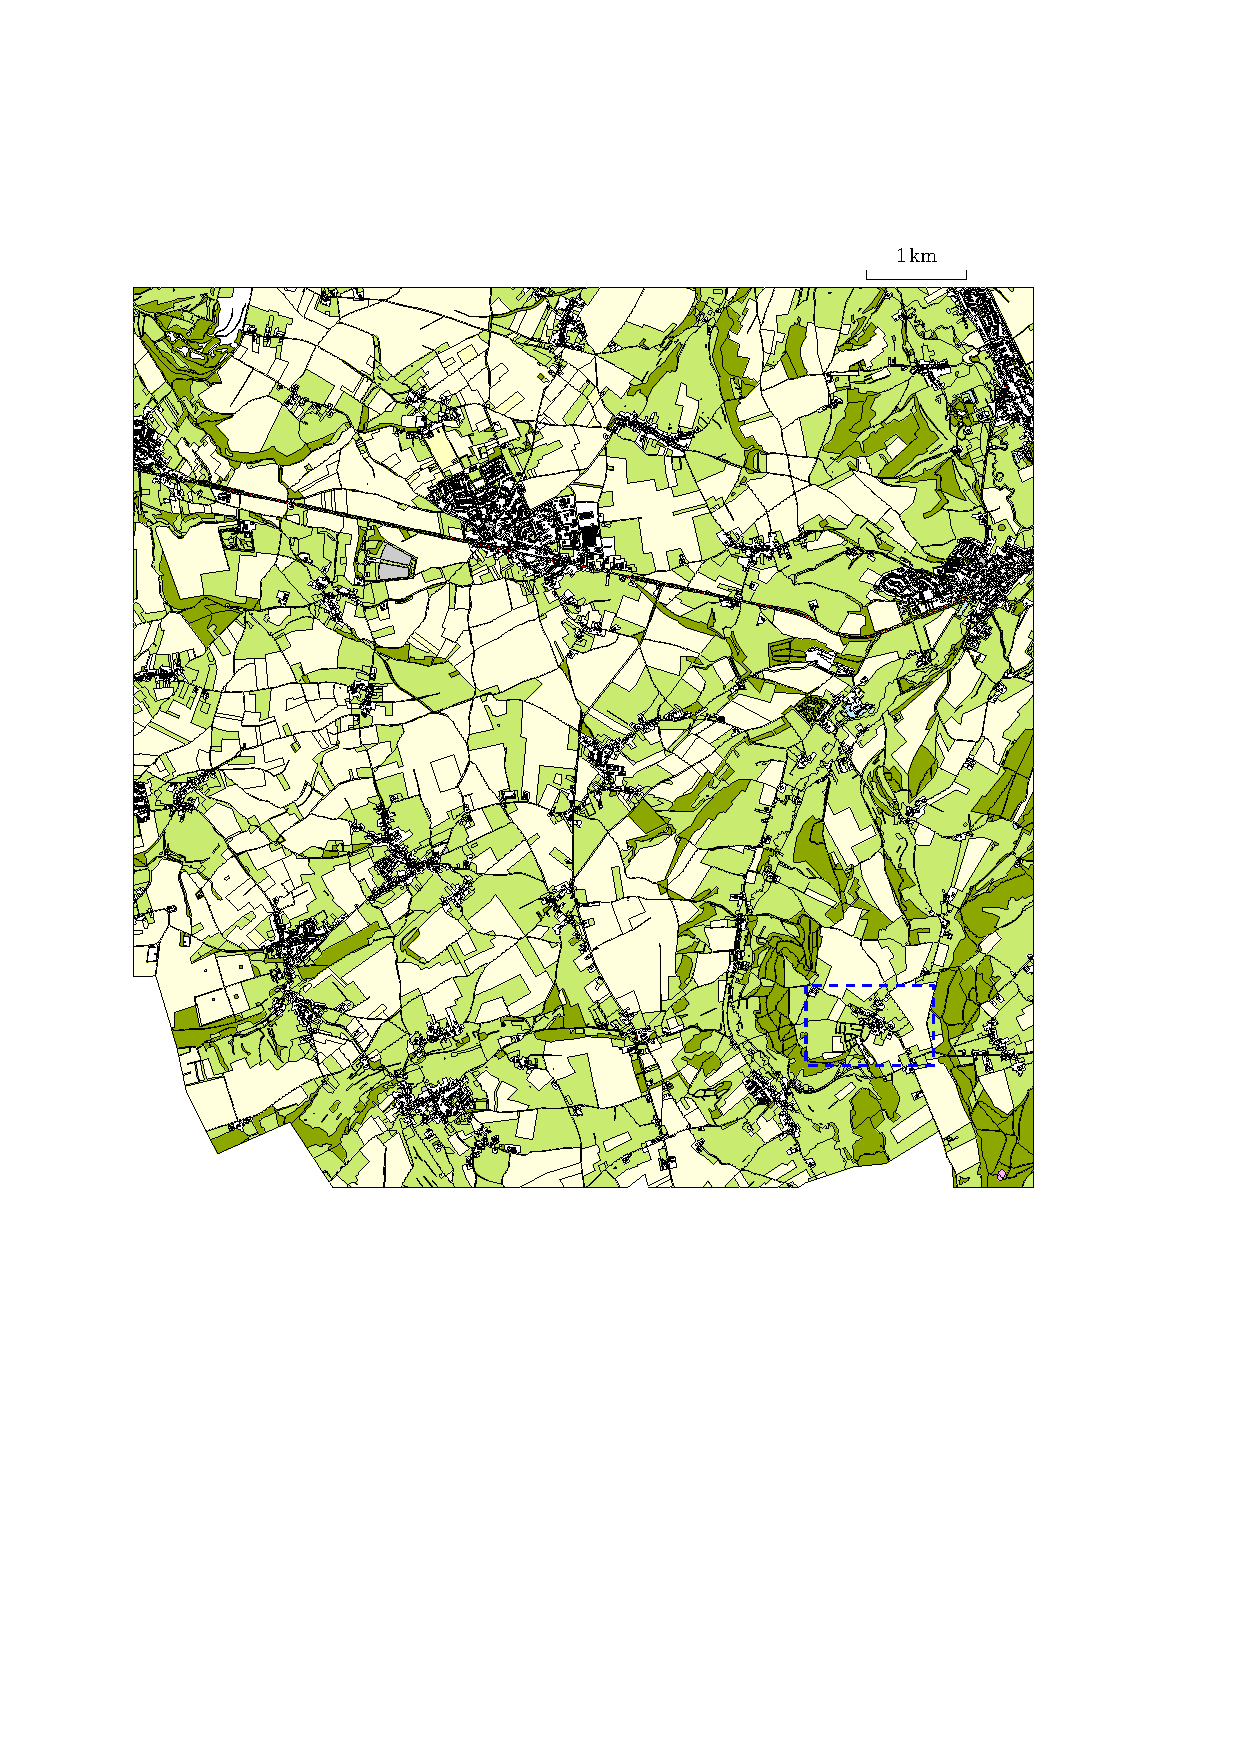
\includegraphics[page=1,draft=false,width=\linewidth,clip=true, trim = 12mm 14mm 2mm 0mm]{data}
%\caption{
%    The topographic map represents the place 
%    in the south of Limburg, The Netherlands.
%    There are $13{,}238$ parcels.
%    The map is for scale $1:10{,}000$.}
%\label{fig:data}
%\end{figure}
%
%
%\begin{figure*}[tb]
%\centering
%\begin{subfigure}[t]{0.48\textwidth}
%\centering
%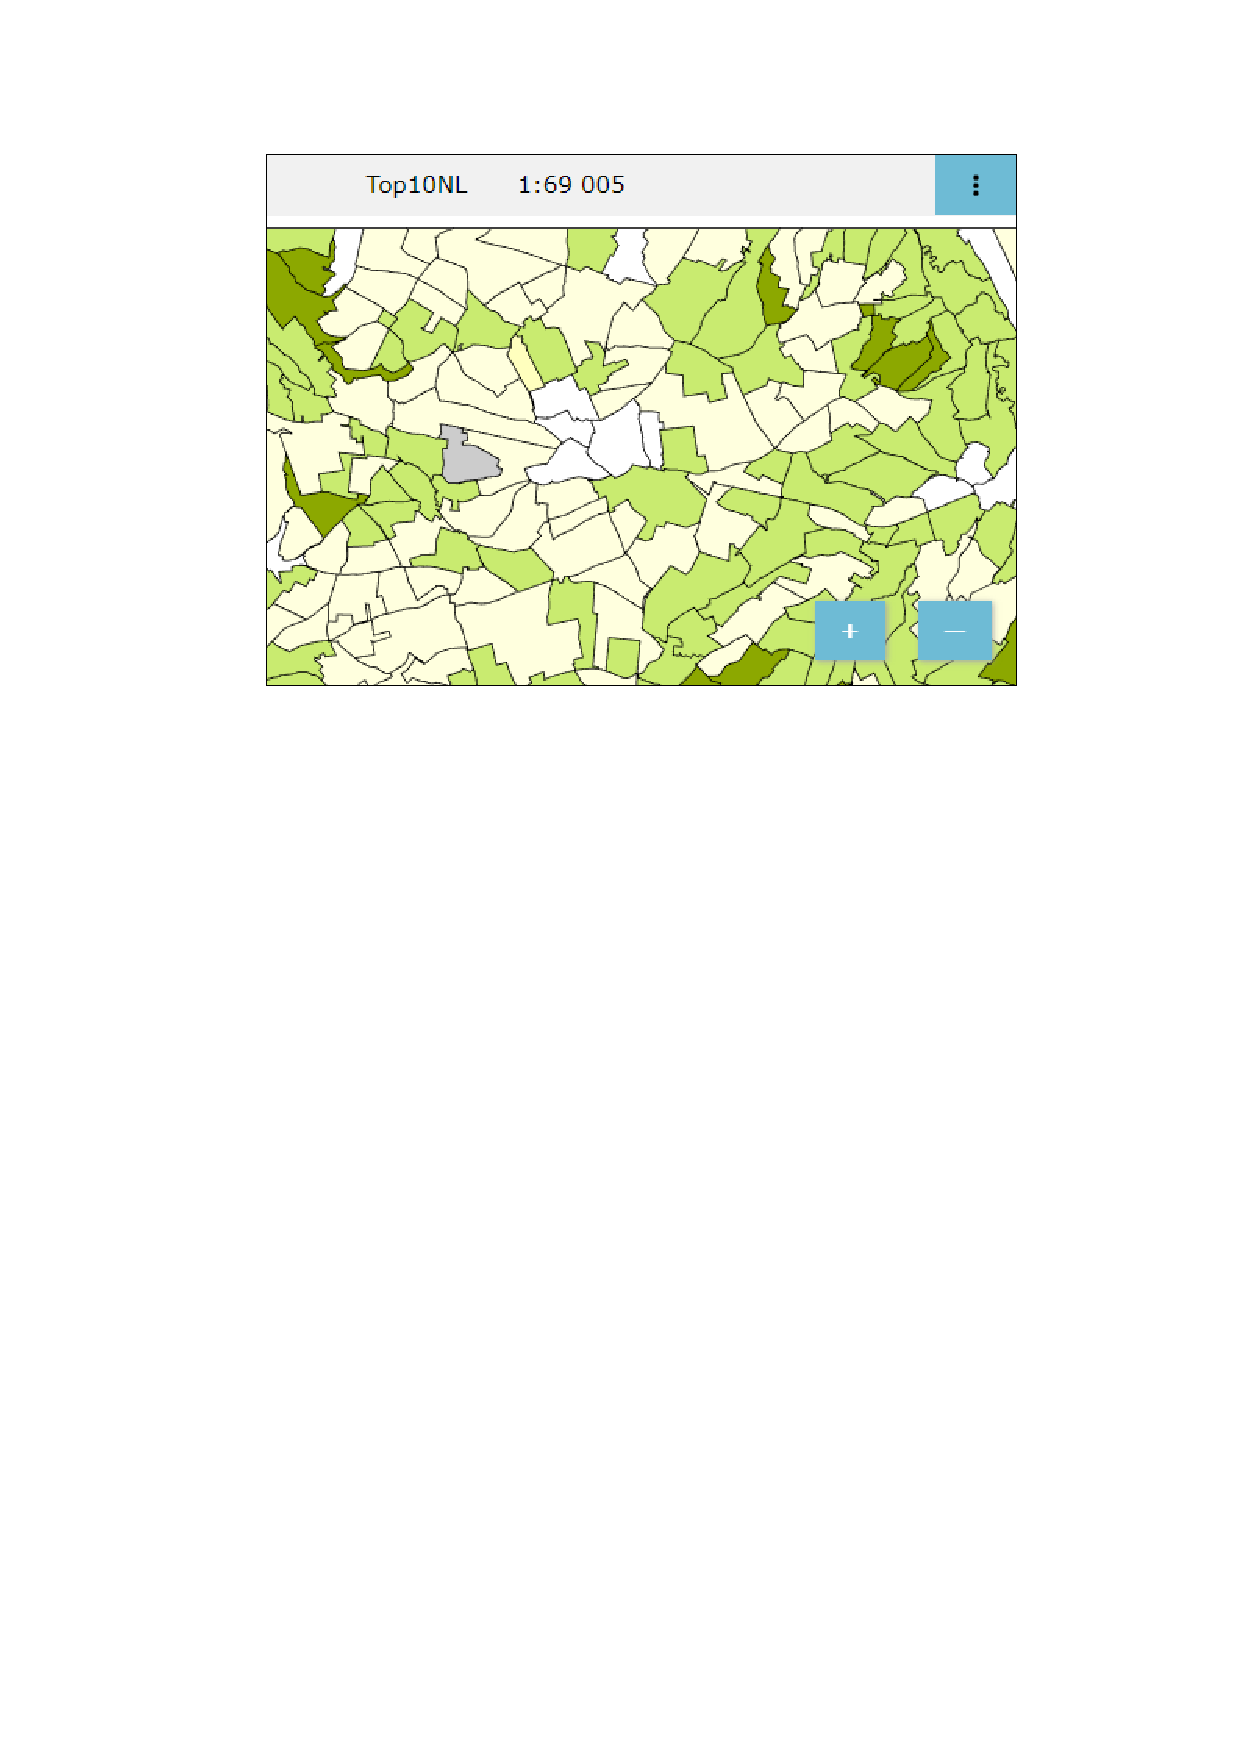
\includegraphics[page=1,scale=0.6]{case_study}
%\caption{An overview map. The map is generated from the base map 
%    by parallel merging with parameter~$r_\mathrm{parallel}= 0.01$.}
%\end{subfigure}
%%\newline
%%\vspace{0.5cm}
%%
%\hfill
%\begin{subfigure}[t]{0.48\textwidth}
%\centering
%\includegraphics[page=2,scale=0.6]{case_study}
%\caption{A part of the base map. The displayed place is marked 
%    by the dashed rectangle in \fig\ref{fig:data}.}
%\end{subfigure}
%\caption{Two examples of our web map with different scales.
%    }
%\label{fig:web_map}
%\end{figure*}
%
%
%%\begin{figure*}
%%\centering
%%\begin{subfigure}[t]{0.48\textwidth}
%%\centering
%%\includegraphics[page=4,width=0.95\linewidth]{methodology}
%%\caption{The SSC of the single merging of \figs\ref{fig:intro}d--j.}
%%\end{subfigure}
%%\hfill
%%\begin{subfigure}[t]{0.48\textwidth}
%%\centering
%%\includegraphics[page=5,width=0.95\linewidth]{methodology}
%%\caption{The SSC of the parallel merging of \figs\ref{fig:intro}k--o}
%%\end{subfigure}
%%\caption{
%%In the left SSC, only one merging event is happening 
%%at a specific state ($z$-dimension), 
%%while in the right SSC multiple merging events may happen at the same state.
%%}
%%\label{fig:ssc}
%%\end{figure*}
%
%Some statistics of the results when 
%parallel parameter~$r_\mathrm{parallel}=0.001$, $0.01$, or $0.1$ 
%are shown in \tbl\ref{tbl:parallel_param_comparison}.
%According to column~$N_\mathrm{step}$,
%the number of steps decreases 
%when the parallel parameter increases.
%This is reasonable because more areas will be merged in each step.
%As explained in \sect\ref{sec:greedy_algo}, 
%for each merging step we iteratively select the least important area 
%and its most compatible neighbor to define a merging event; 
%then, we block the neighbors of the two areas.
%Sometimes, a least important area is already blocked 
%because of the previously found events.
%This situation happens~$2{,}714$ times in total for all the steps
%when parallel parameter~$r_\mathrm{parallel}=0.01$
%(see column~$N_\mathrm{blocked}$ of \tbl\ref{tbl:parallel_param_comparison}).
%%
%Sometimes, although a least important area is free, 
%its most compatible neighbor has been blocked 
%because of the previously found events.
%This case happens~$1{,}383$ times in total for all the steps
%when parallel parameter~$r_\mathrm{parallel}=0.01$
%(see column~$n_\mathrm{nbr\_blocked}$ of \tbl\ref{tbl:parallel_param_comparison}).
%%
%According to the statistics, we encounter more cases of the areas blocked
%when merging a larger proportion of the area objects.
%However, we can still reach our target number of events perfectly 
%for settings of~$r_\mathrm{parallel}=0.01$ or~$r_\mathrm{parallel}=0.001$. 
%Only when we push beyond the limit (\eg~$r_\mathrm{parallel}=0.1$), 
%we can not reach the target number of events in a step 
%(and we need correction information 
%to compute the actual number of achieved events). 
%When the target number of events cannot be met, 
%one could also question the cartographic quality 
%if there is hardly any free choice when generalizing.
%
%
%\begin{table}[tb]
%\centering
%\caption{Some statistics when different parallel parameters area used 
%    (\ie~$r_\mathrm{parallel}=0.001$, $0.01$, and $0.1$).
%    Column~$N_\mathrm{step}$ records the number of steps to transit 
%    from the base map to the map with a single area.    
%    Column~$N_\mathrm{blocked}$ records the number of times
%    when the least important area was blocked.
%    Column~$N_\mathrm{nbr\_blocked}$ records the number of times 
%    when the most compatible neighbor was blocked.
%}
%\begin{tabular}{rrrr}
%\toprule
%$r_\mathrm{parallel}$   & $N_\mathrm{step}$ & $N_\mathrm{blocked}$  & $N_\mathrm{nbr\_blocked}$ \\ \midrule
%0.001                   &  3{,}195          &       211             &       72                  \\
%0.01                    &  544              &   2{,}714             &  1{,}383                  \\
%0.1                     &  91               & 100{,}617             & 34{,}268                  \\ 
%\bottomrule 
%\end{tabular}
%%\begin{tabular}{cccc}
%%\hline
%%$r_\mathrm{parallel}$ & 0.001       & 0.01          & 0.1    \\ \hline
%%eventdiff\_repetition & [[0, 3195]] & [[0, 544]]    & $L_{\mathrm{diff\_rep}, 0.1}$   \\
%%least face blocked    & 228            & 3{,}216         & 105{,}980       \\
%%best neighbor blocked & 72            & 1{,}841        & 38{,}232 \\ \hline 
%%\end{tabular}
%%\begin{Verbatim}[fontfamily=normal,commandchars=\\\{\},
%%codes={\catcode`$=3\catcode`^=7\catcode`_=8}]
%%\hspace{4cm}$L_{\mathrm{step\_eventdiff},0.1}$ = [[1, 53], [2, 138], $\dots$, [88, 1]]
%%\end{Verbatim}
%%\fvset{gobble=2}
%%\begin{Verbatim}[fontfamily=normal,frame=single,
%%label=$L_{\mathrm{diff\_rep}, 0.1}$]
%%   [[51, 1], [138, 1], [152, 1], [200, 1], [205, 1], [181, 1], [198, 1], [167, 1], [173, 1], [165, 1], 
%%    [153, 1], [143, 1], [140, 1], [127, 1], [125, 1], [108, 1], [103, 1], [92, 2], [84, 1], [79, 1], [74, 1], [68, 1], 
%%    [60, 1], [54, 1], [46, 1], [50, 1], [48, 1], [45, 1], [39, 1], [44, 1], [37, 1], [36, 1], [32, 1], [30, 1], [26, 1], 
%%    [28, 1], [21, 2], [18, 1], [20, 1], [16, 1], [12, 1], [13, 1], [8, 1], [12, 2], [6, 1], [12, 1], [11, 1], [8, 1], [7, 1], 
%%    [6, 1], [7, 1], [4, 1], [5, 1], [4, 1], [5, 2], [7, 1], [5, 1], [4, 1], [5, 1], [3, 1], [4, 1], [3, 3], [2, 2], [1, 2], [2, 1], 
%%    [1, 2], [2, 1], [1, 3], [0, 2], [1, 2], [0, 14]]
%%\end{Verbatim}
%\label{tbl:parallel_param_comparison}
%\end{table}
%
%
%
%As we can find the target numbers of merging events for all the steps
%when parallel parameter $r_\mathrm{parallel}= 0.001$ or~$0.01$, 
%the corresponding exceptions lists are empty.
%%For example, when~$r_\mathrm{parallel}= 0.01$,
%%The content of the JSON file is as following.
%%\begin{verbatim}
%%                {
%%                    "face_num": 13238,
%%                    "parallel_param": 0.01,                    
%%                    "step_eventdiff": []
%%                }
%%\end{verbatim}
%When $r_\mathrm{parallel}= 0.1$,
%the exception list is~$[[1, 1304], [2, 1070], \dots, [77, 2]]$,
%which has~$71$ pairs of values.
%In reality, we would not use~$r_\mathrm{parallel}= 0.1$
%(merging~$10\%$ of the current areas in every step)
%because it is an unrealistic high value.
%Using such a high value results in a multi-scale representation
%(because we have a few valid states or scales),
%whereas we would like to have representations at nearly
%arbitrary scales.
%
%%Important note: this is for a small subset 9x9 out of the 300x300 km^2 (whole country). To have same effect can we keep the r_parellel at same value, but we will have less situation where the target is not reached (more options)
%
%
%
%We set zooming factor~$f_\mathrm{zoom}=1$ and 
%zooming duration~$t_\mathrm{zoom}=1 s$ 
%(see \sect\ref{sec:zooming_duration}).
%When zooming on our web maps with different parallel parameters,
%we observed that the impressions of the maps 
%based on single merging\footnote{%
%See the web map at
%\url{https://congengis.github.io/webmaps/2020/05/merge/single-merging/}.} 
%and based on parallel merging with parameter~$r_\mathrm{parallel}= 0.001$ 
%are almost the same.
%The reason is that the smooth merging happens too fast,
%and we cannot really see the merging animation.
%We get the feeling of smooth merging when~$r_\mathrm{parallel}= 0.01$.
%When~$r_\mathrm{parallel}= 0.1$, the smooth merging is already obvious.
%In order to show a better comparison of single merging 
%and parallel merging,
%we put two maps together (see \fig\ref{fig:comparison}),
%where the parallel parameter is~$0.1$.\footnote{%
%See the map of comparison at
%\url{https://congengis.github.io/webmaps/2020/05/merge/0.1/comparer.html}.}  
%
%
%\begin{figure}[tb]
%\centering
%\includegraphics[page=3,scale=0.6]{case_study}
%\caption{
%    The map to the left of the slider is based on single merging,
%    and the one to the right is based on parallel merging
%    with~$r_\mathrm{parallel}= 0.1$.
%    The slider can be moved to tune the widths of the two map canvases.
%    The two maps are very different, and 
%    we can observe some sudden changes across the slider.
%}
%\label{fig:comparison}
%\end{figure}
%
%When parallel parameter~$r_\mathrm{parallel}$ is set to~$0.1$,
%we noticed a problem in the northeastern corner of the map.
%That is, some tiny and relatively unimportant areas stay 
%until the scale is very small,
%while they should be merged much earlier.
%This is due to the fact that 
%there are many buildings in the northeastern corner of the map.
%When the buildings share the same surrounding area,
%they become holes of the polygon.
%In each step, only one of the buildings will be merged into the surrounding area
%because an area is allowed to merge with only one area in each step.
%In the meantime, the areas at other places of the map merge relatively fast
%because we allow $10\%$ of the areas to be merged in each step.
%Fortunately, we would not need to use such a big parallel parameter in reality.




\section{Concluding remarks}
\label{sec:concluding_remarks}

This paper investigates on paralleling generalization operations,
using the merging operation as a case study. 
According to our experiment,
the events of parallel merging 
can be better observed than the events of single merging.
This result shows the potential that,
when zooming on a map based on parallel-event operations,
users can keep their context better 
and can have smoother map interaction experience.

Many topics related to this research need to be investigated further.
We need to test our method on a topographic map with much more objects,
In that case, the client side will need to dynamically load 
and process the map data 
for the place and the scale being viewed.
The client also needs to remove the loaded data that is not used for a while 
in order to release memory.
With those functionalities, our prototype will be able to handle 
a map with arbitrary number of area objects.
Our current event consists of only the merging operation,
it is also necessary to involve split operation
because sometimes a merging operation results in an unnatural area
\citep{Haunert2008Skeleton,Meijers2016Split}.
To avoid clutter of vertices for zooming out, 
it is necessary to simplify the boundaries of the areas.
Many existing methods could be integrated into our parallel paradigm.
\citet{Meijers2011LineSimp} proposed a method 
to simplify the boundaries parallelly. 
Their results are topologically safe. 
Another future work is to investigate 
how much map users benefit from our parallel merging.
We need to conduct some usability tests based on the experience of
\citet[\sect6.7]{Suba2017Thesis} and \citet{Midtbo2007}.
We currently drive the merging by the relationship 
between the number of areas and the scale;
an other strategy is to drive 
by the relationship between the size of the smallest area and the scale.
We also need to test which of the two strategies is better.


%\subsection{Conclusion}
%%For the first time, 
%This paper investigates on paralleling generalization operations,
%using the merging operation as a case study. 
%The purpose of having parallel generalization operations 
%is to have smoother zooming experience later on 
%(compared to the pure sequenced individual generalization events)
%so that users can better keep their context during zooming.
%This paper develops a greedy algorithm to find parallel events of 
%merging area objects.
%Then, the parallel events are integrated into 
%the tGAP and the SSC to nicely visualize the merging animations.
%%This paper also proposed a strategy 
%%to concisely store the number of merging events for all the steps.
%To guarantee that the merging animations always complete for zooming, 
%we managed to snap zooming operations to valid states.
%This paper also presents a recipe 
%to define the animation duration of an event.
%According to our case study,
%the events of parallel merging 
%can be better observed than the events of single merging.
%This result shows the potential that
%users can keep their context better 
%and can have smoother map interaction experience
%when zooming on a map based on parallel-event operations.
%
%
%
%\subsection{Future work}
%
%
%
%
%Many topics related to this research need to be investigated further.
%The case study with $13{,}238$ area objects 
%demonstrated the efficiency of our map.
%For a topographic map with much more objects,
%we will need to make $3$-d tiles of the map data.
%Then, the client side will dynamically load and process the map data 
%for the place and the scale being viewed.
%The client also needs to remove the loaded data that is not used for a while 
%in order to release memory.
%With those functionalities, our prototype will be able to handle 
%a map with arbitrary number of area objects.
%Those functionalities are under development 
%and will be presented in another paper.
%
%
%\fig\ref{fig:smooth_merging}a--e shows our solution of
%gradually expanding an area over the other area.
%It may be even better if the color of the smaller area (pink)
%adapts to the color of the larger one (light yellow) smoothly
%(see \fig\ref{fig:smooth_merging}f--j).
%
%
%\begin{figure*}[tb]
%\centering
%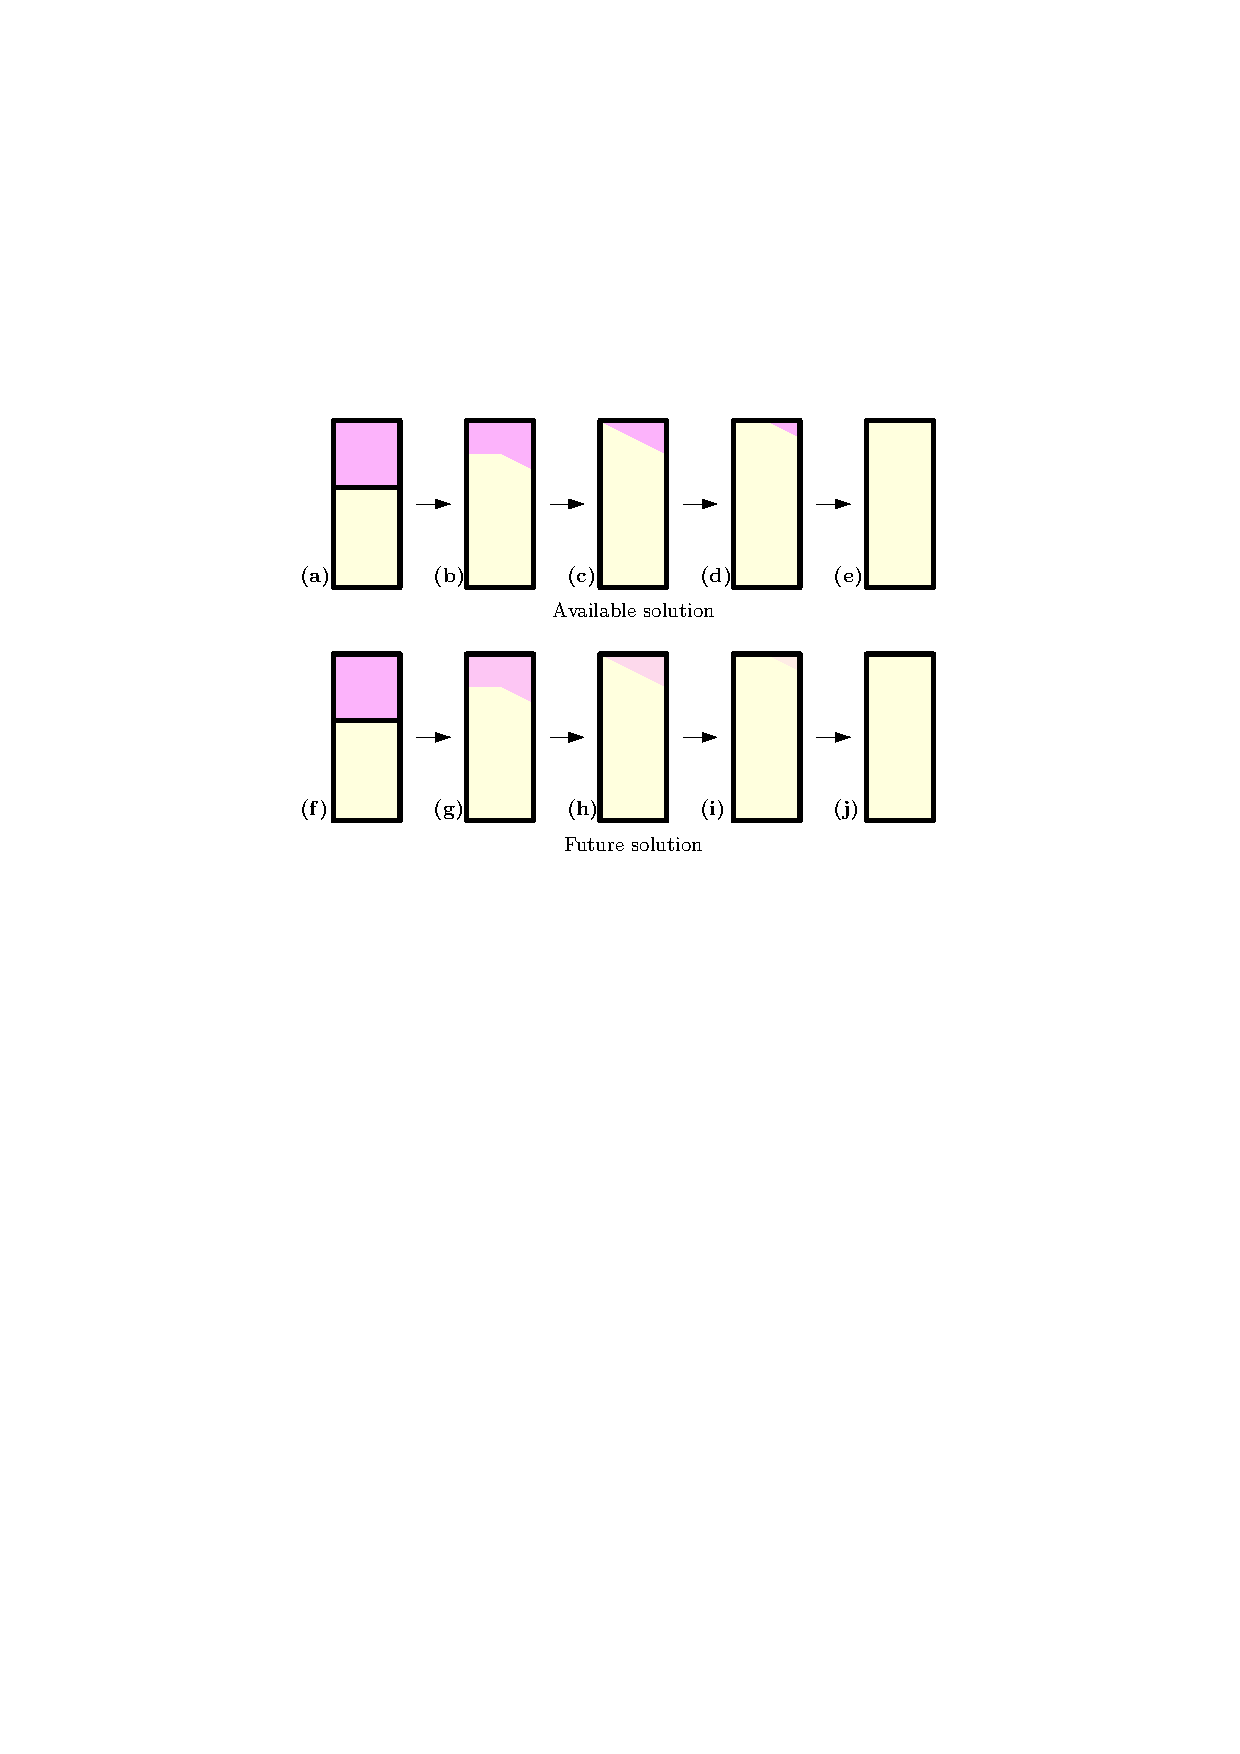
\includegraphics[page=1]{concluding_remarks}
%\caption{
%    Our available solution of merging animation 
%    and a possible future solution.}
%\label{fig:smooth_merging}
%\end{figure*}
%
%
%
%%\begin{figure}[tb]
%%\centering
%%\includegraphics[page=1]{smooth_merging}
%%\caption{A smooth way of merging two areas,
%%    where the larger area gradually expands over the smaller one.}
%%\label{fig:smooth_merging}
%%%
%%\vspace{6mm}
%%%
%%\centering
%%\includegraphics[page=2, scale=0.3]{smooth_merging}
%%\caption{The space-scale cube for the merging 
%%    of \fig\ref{fig:smooth_merging}.
%%    This figure is made by visualizing the content of an obj file in 
%%    ParaView 5.6.0.}
%%\label{fig:smooth_merging_ssc}
%%\end{figure}
%
%
%
%
%This paper used a greedy algorithm 
%to find parallel merging events for each step.
%Alternatively, it is possible to define merging steps 
%by selecting and combining some single-event steps of a sequence found 
%by some existing methods
%(\eg~the greedy algorithm of \citet{vanOosterom2005}
%or the \Astar algorithm of \citet[\chap2]{Peng2019Thesis}).
%
%Currently, the merging events distribute randomly on a map.
%If we are unlucky, there may be a lot of events 
%happening in users' focused region for a zooming duration,
%which may cause the users to lose track of their interested objects;
%for another zooming duration, 
%there may be no event happening in the focused region at all.
%The strategy of blocking neighbor areas in our greedy algorithm 
%already mitigates the problem.
%However, it may be even better if 
%we explicitly distribute the merging events evenly, 
%then the workload for a user to follow the events is stable during the zooming.
%To this end, we could divide a map into many regions 
%using a field-tree-like, multiple-level grid \citep{vanPutten1998NewGAP}
%or using the road network.
%Then, we could find a certain number of events in each of the regions 
%according to the regions' sizes,
%which should result in an even distribution of events.
%Finally, we could compare our current greedy algorithm and 
%the algorithm considering even distribution.
%
%If some small parcels distribute at a large region,
%then the background parcel will eat all the small parcels.
%This case already happens in our web maps
%when some small buildings are inside a settlement area.
%In order to solve this problem, 
%we could generate a tessellation of the small parcels
%using the method of \citet{Ai2015Building}.
%Then, we could grow each of the small parcels 
%inside its own cell.
%By then, the small parcels will touch each other
%and can be merged by eating each other.
%
%Our current event consists of only the merging operation,
%it is also necessary to involve split operation
%because sometimes a merging operation results in an unnatural area.
%For example, it is weird to merge a long and thin area 
%with one of the areas that are along it
%\citep[see][]{Haunert2008Skeleton}.
%Therefore, such kind of long and thin areas should be
%split into several parts first.
%We may integrate a split method based on the straight skeleton
%\citep{Haunert2008Skeleton}
%or the skeleton obtained from a constrained Delaunay triangulation
%\citep{Meijers2016Split}.
%In addition to area features, we also need to support line features 
%for these long objects (\eg~roads, river, rail) for the smaller scales.
%In order to apply appropriate generalization operators
%for a certain scale,
%we need to extend and implement the framework 
%to guide our generalization choices
%\citep{Meijers2018Framework}.
%
%
%To avoid clutter of vertices for zooming out, 
%it is necessary to simplify the boundaries of the areas.
%Many existing methods could be integrated into our parallel paradigm.
%\citet{Meijers2011LineSimp} proposed a method 
%to simplify the boundaries parallelly. 
%Their results are topologically safe. 
%Another choice would be the method of \citet{ImaiIri1988},
%which is able to minimize the number of vertices 
%for a given error threshold.
%One more choice would be to construct compatible triangulations 
%\citep[see][\chap3]{Peng2019Thesis}
%for the two levels of topographic maps.
%In the SSC, we could build some tilted walls 
%to connect the two levels of compatible triangulations.
%When we slice this SSC to animate a zooming action,
%the boundaries of the areas are morphed 
%(moved smoothly and parallelly)
%between a detailed representation and a coarse representation.
%We can imagine that it is challenging to build the tilted walls.
%Furthermore, we would like to 
%simplify point symbols and text labels in a smooth way.
%For this purpose, we may need to integrate the ideas of
%\citet{Haunert2017Label} and \citet{sahw-oarps-ICAGW13}.
%
%We would also like to realize smooth zooming
%between a foreground map and a background map,
%which respectively present a thematic data and a topographical data.
%When a user zooms in, the foreground map should be displayed,
%and when the user zooms out,
%the background map should be displayed.
%Furthermore, we would like to 
%integrate time dimension into our 3-dimensional SSC
%to form a 4-dimensional space-scale-time structure (a tesseract).
%Then, we have the opportunity to store all the updates along time in the tesseract.
%By ``slicing'' it, we will be able to output a map at any scale and any time point.
%
%
%This paper develops the technique for smooth zooming based on parallel merging,
%and we hope that it allows map users to follow the zooming more easily.
%A future work is to investigate 
%how much map users benefit from our technique.
%We will conduct some usability tests based on the experience of
%\citet[\sect6.7]{Suba2017Thesis} and \citet{Midtbo2007}.
%Another future work is to find optimal parallel parameters for 
%different kinds of datasets.







%When we remove a triangle by slicing the SSC, 
%we may want to keep three vertices of the triangle 
%instead of making four vertices.
%In this case, the polyhedron (with five faces) should have curly edges,
%which is also known as a \emph{curved polyhedron}.
%The slopes of curly edges need to be studied.


%Some research questions are as follows.
%What aspects should we optimize 
%(\eg~minimizing the number of merging events or 
%assigning similar numbers of merging steps to each event)?
%What algorithm should we use 
%(\eg~dynamic programming, \Astar, or integer linear programming)?
%How much time is gained for users to observe the merging steps on the screen?
%How to store the parallel merging steps?




%\section*{Data and codes availability statement}
%
%The data and codes used in this case study 
%can be found at \emph{figshare} 
%(see \url{https://figshare.com/s/199e049e2a0f9c18d19a}).
%The data was derived from open-access dataset TOP10NL,
%which is a topographic map produced by Kadaster
%(see \url{https://www.pdok.nl/downloads/-/article/basisregistratie-topografie-brt-topnl}).
%\footnote{%
%Dataset TOP10NL can be downloaded at
%\url{https://www.pdok.nl/downloads/-/article/basisregistratie-topografie-brt-topnl},
%accessed: May 17, 2020.}

%\subsection{Acknowledgements (optional)}
%Acknowledgements of support for the project / paper / author are welcome.
%
%\subsection{Appendix (optional)}
%Any additional supporting data may be appended, provided the paper does not exceed the limits given above.

% references are included using your bibliography file (*.bib))

\begin{spacing}{0.9}% tune the size by altering the parameter
      \bibliography{Reference/BibReference} % Include your own bibliography (*.bib)
\end{spacing}

\label{LastPage} % added 13-03-2018 by Juergen Bierwirth to get the \pageref{LastPage} result (page numbering in the header)
\end{document}
